\begin{center}
\section*{PHẦN 2: CHI TIẾT DỰ ÁN}
\addcontentsline{toc}{section}{PHẦN 2: CHI TIẾT DỰ ÁN}
\end{center}

\section{Đăng nhập đăng kí}
\subsection{Màn hình đăng nhập tài khoản}
Màn hình đăng nhập cho phép người dùng nhập email và mật khẩu để truy cập ứng dụng. Giao diện đơn giản, thân thiện với người dùng, kèm theo xác thực tài khoản thông qua Firebase Authentication. Khi người dùng đăng nhập thành công, ứng dụng sẽ chuyển sang màn hình chính có các chức năng học tập. Ngoài ra, còn hỗ trợ xác thực Google giúp đăng nhập nhanh chóng.
\begin{center}
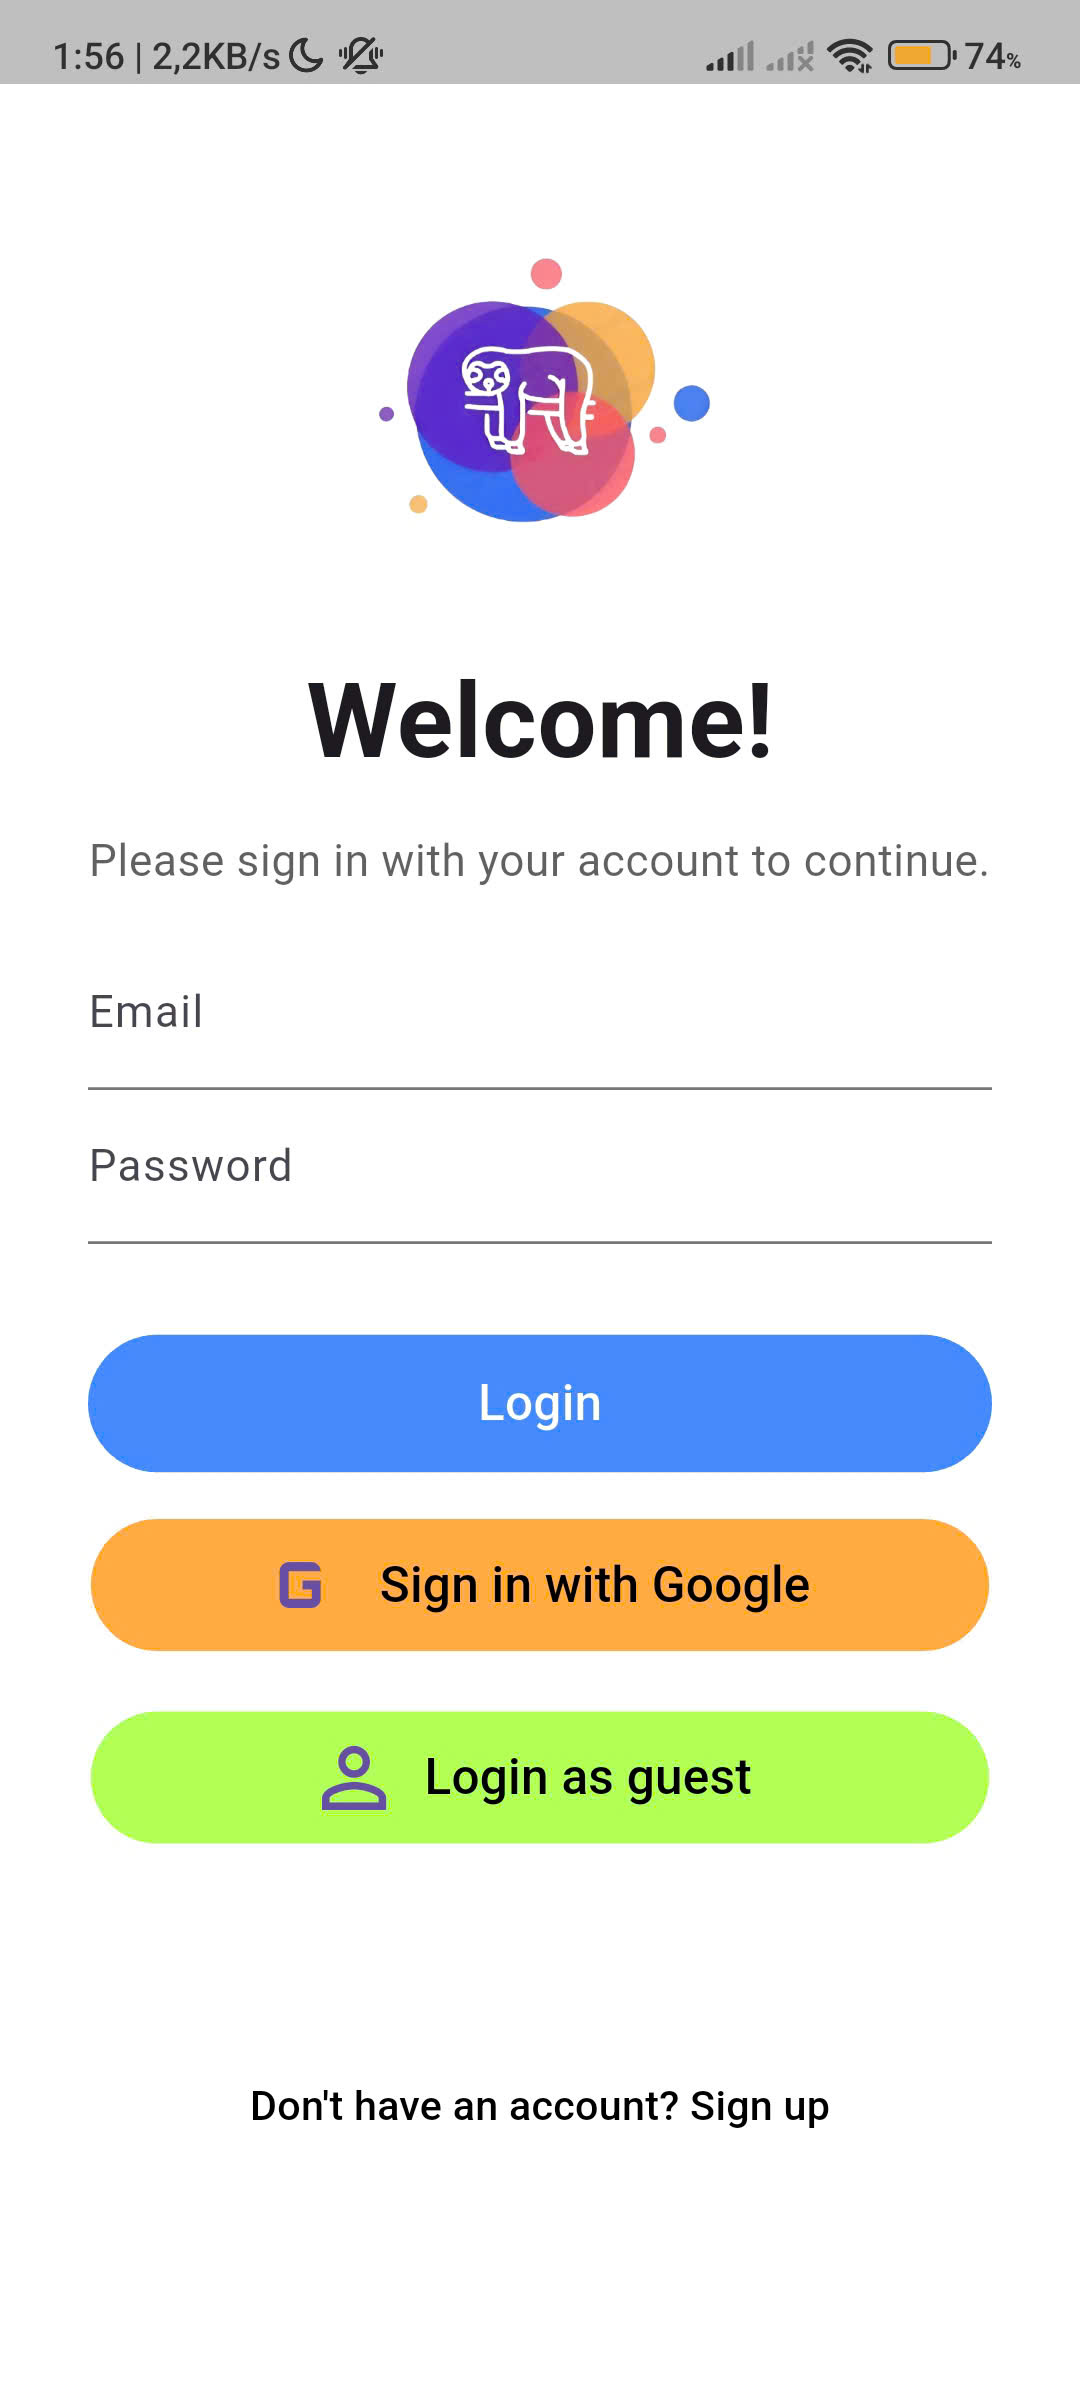
\includegraphics[width=8cm]{ảnh/1.jpg}
\end{center}
 

\subsection{Màn hình đăng kí tài khoản}
Màn hình này cho phép người dùng tạo tài khoản mới bằng email và mật khẩu. Sau khi nhập đầy đủ thông tin hợp lệ, tài khoản được tạo và lưu vào Firebase Authentication. Người dùng sau đó có thể đăng nhập và sử dụng tất cả các tính năng của ứng dụng.
\begin{center}
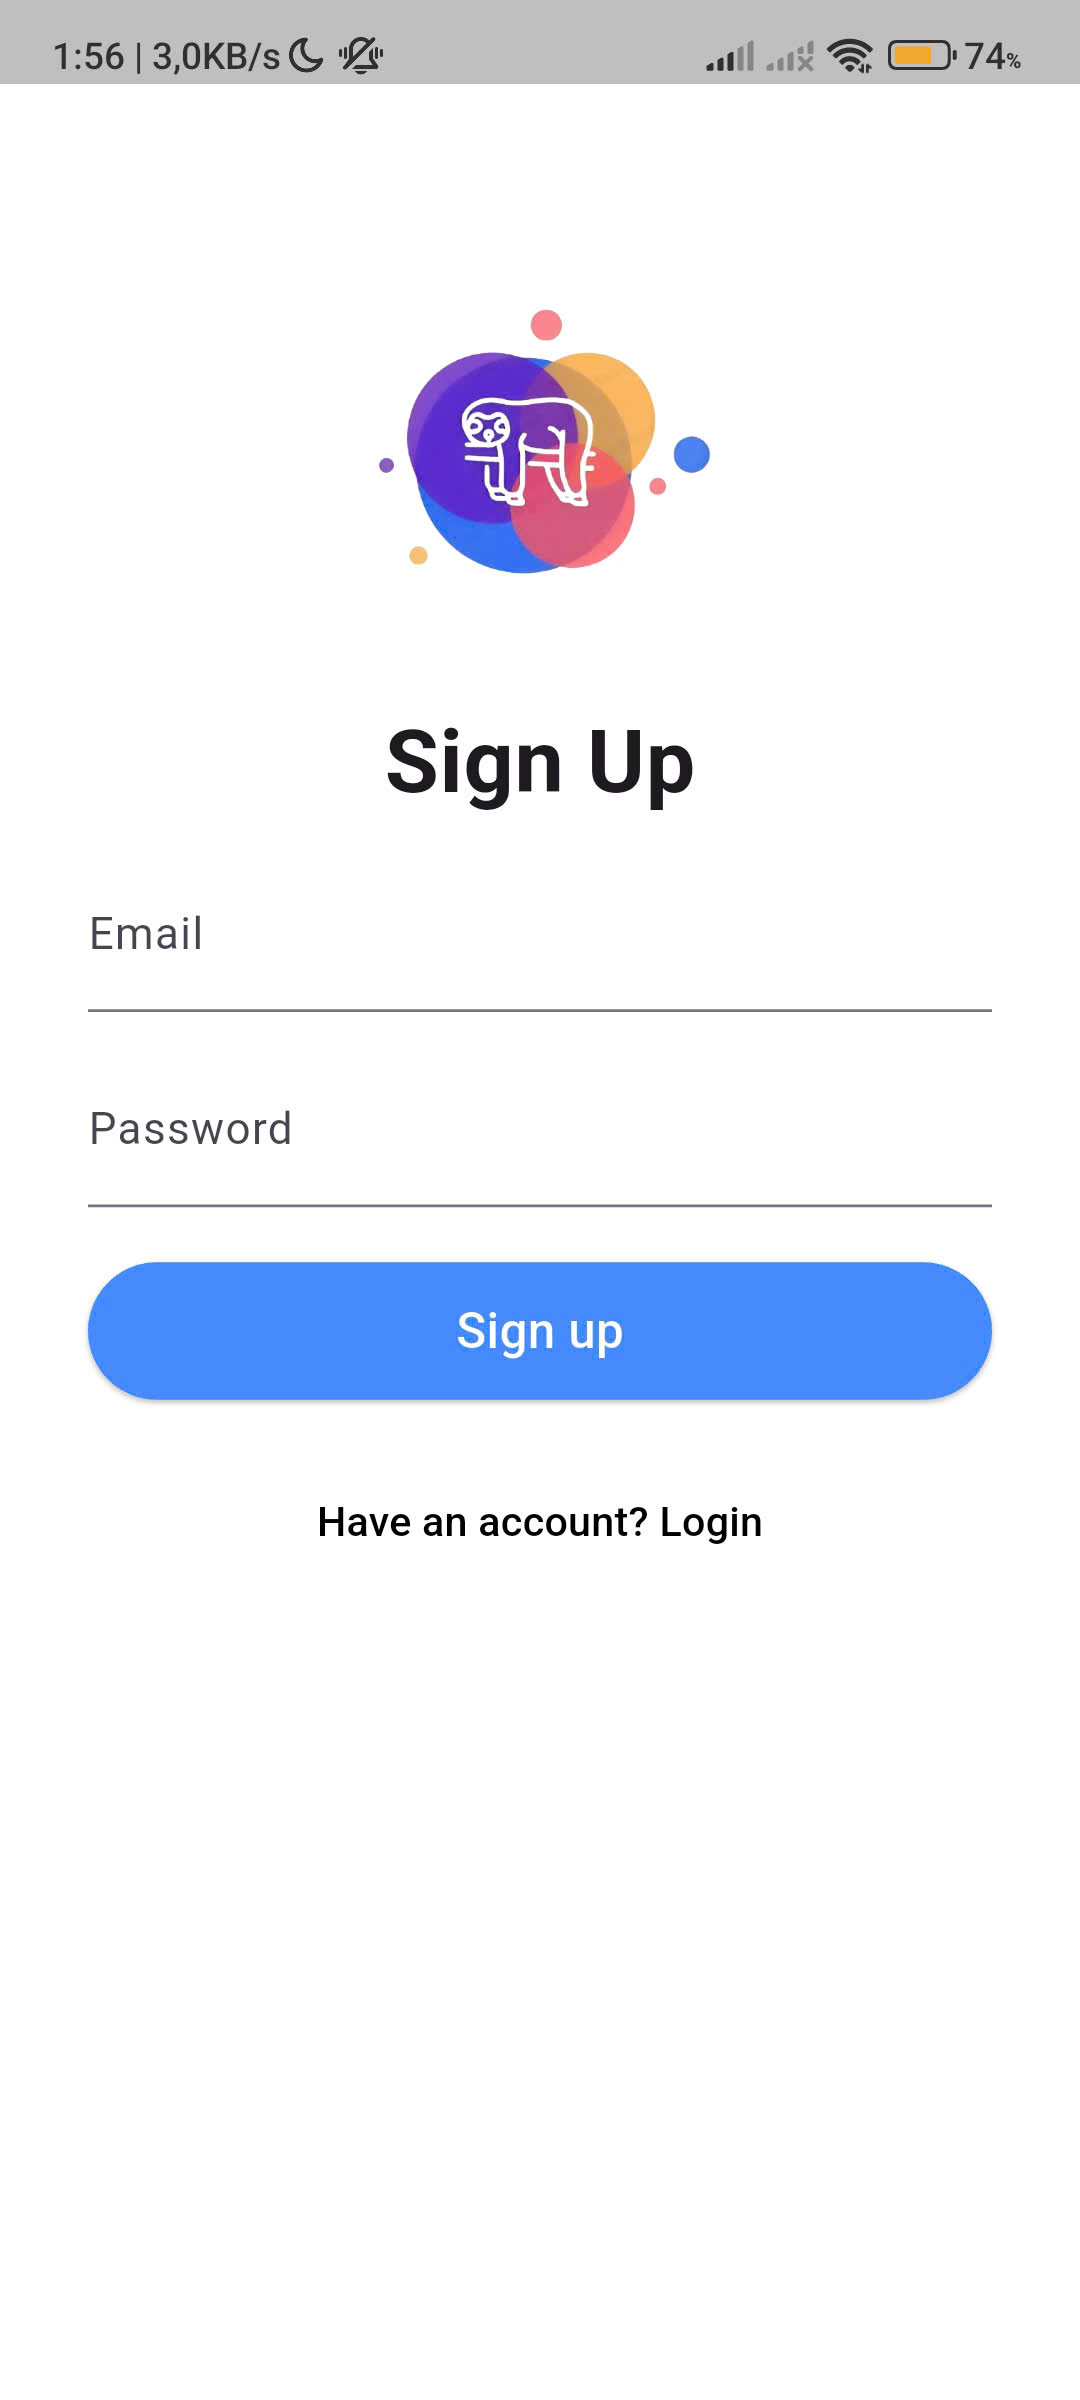
\includegraphics[width=9cm]{ảnh/3.jpg}
\end{center}

\section{Chức năng từ điển}
\subsection{Màn hình từ điển}
Màn hình hiển thị danh sách các từ vựng được lấy từ file json ở local. Mỗi từ bao gồm nghĩa tiếng Việt, phiên âm và khả năng nhấn để xem chi tiết. Giao diện có thanh tìm kiếm, nút bookmark.
\begin{center}
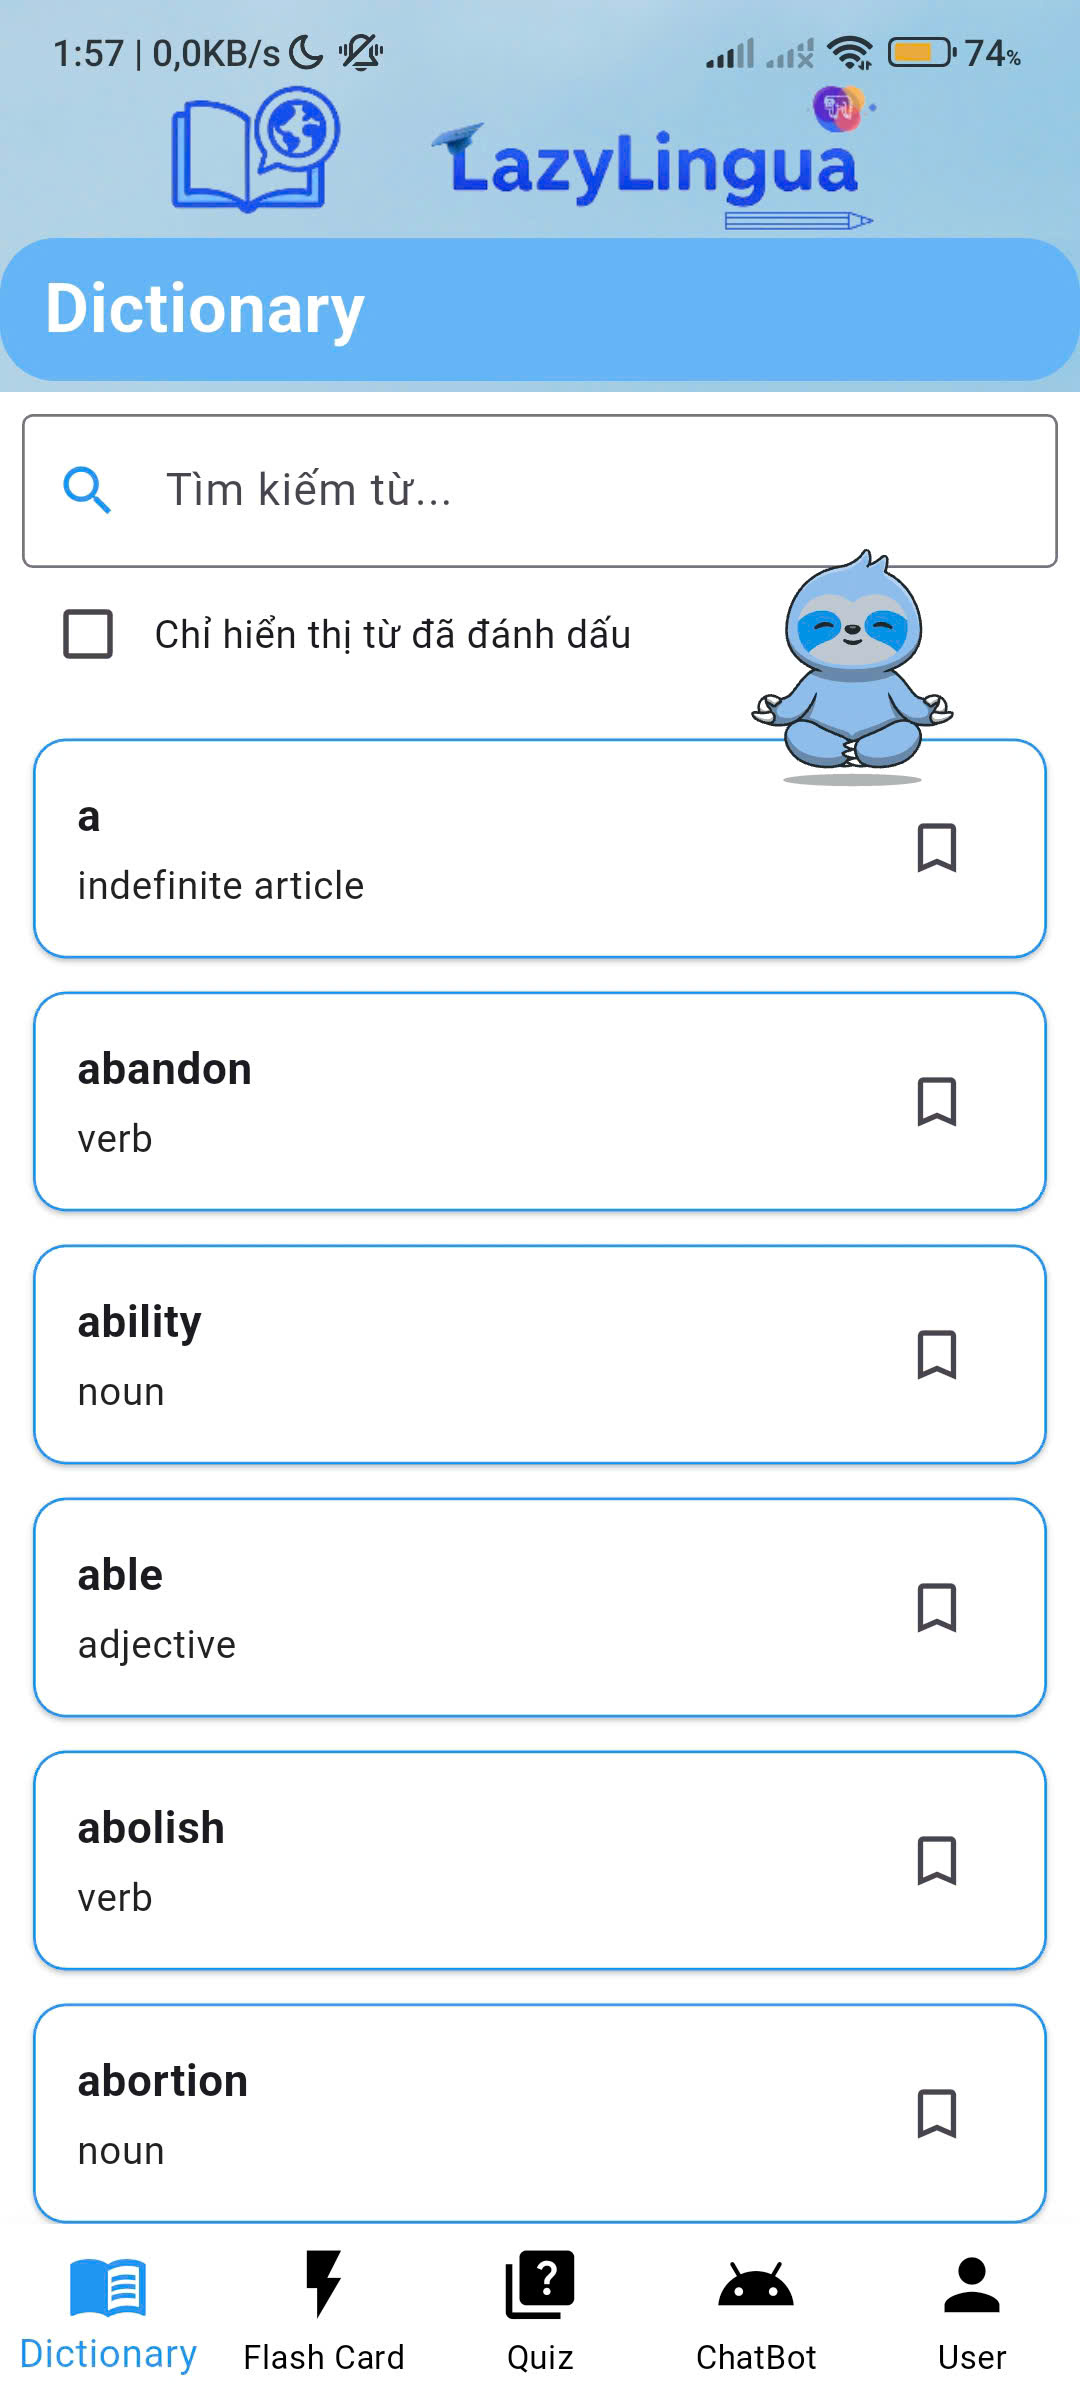
\includegraphics[width=9cm]{ảnh/4.jpg}
\end{center}
\subsection{Tìm kiếm từ}
Chức năng tìm kiếm giúp người dùng nhập từ tiếng Anh cần tra cứu. Kết quả sẽ được lọc theo từ khóa, trả về các từ khớp và hiển thị cùng định nghĩa. Tính năng tìm kiếm được tối ưu để phản hồi nhanh.
\begin{center}
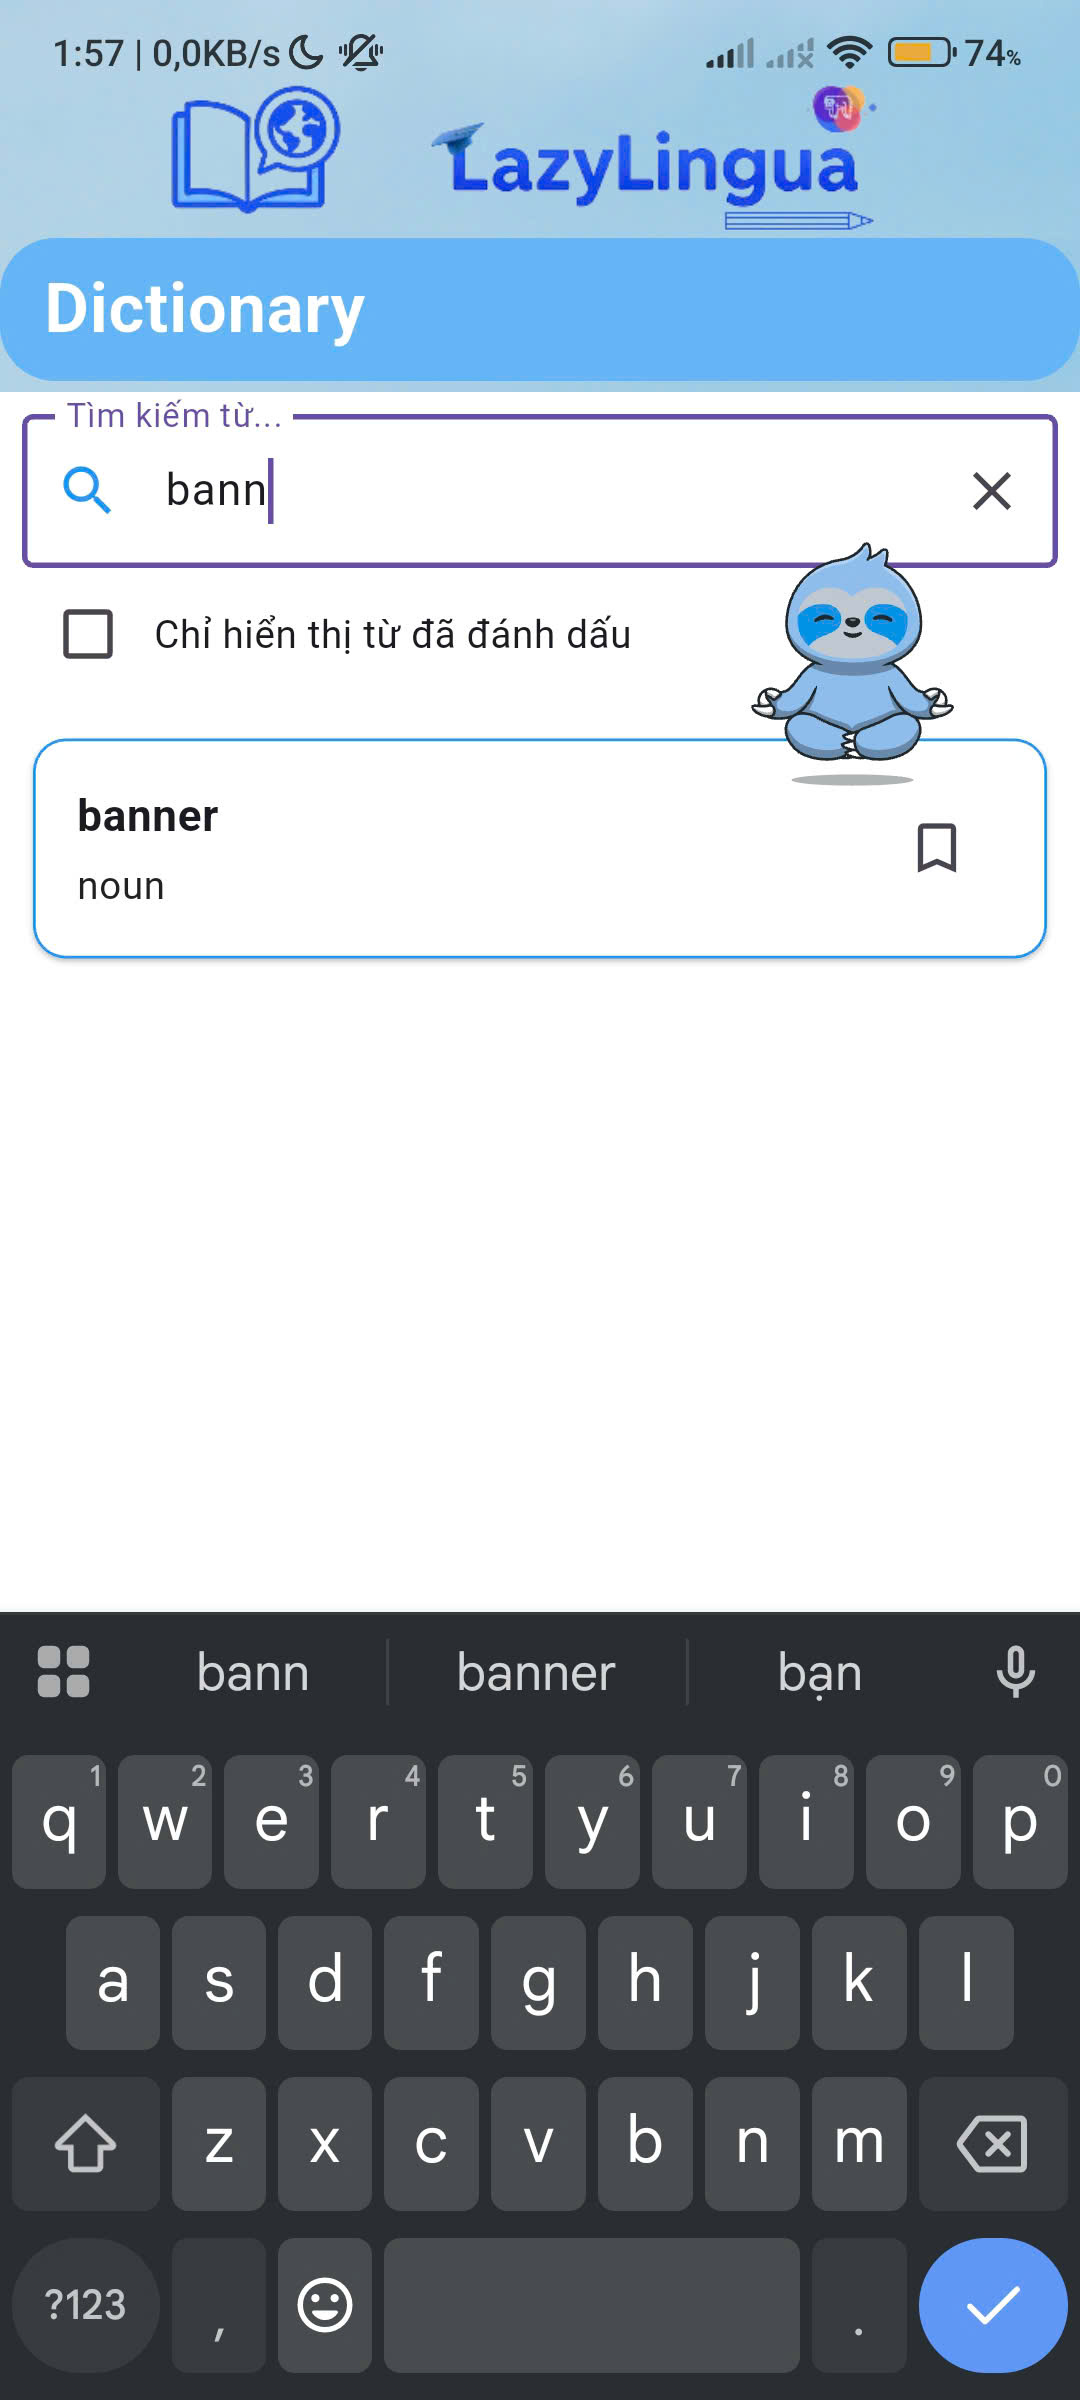
\includegraphics[width=9cm]{ảnh/6.jpg}
\end{center}
\subsection{Bookmark}
Người dùng có thể nhấn vào biểu tượng bookmark để lưu lại các từ vựng yêu thích hoặc đang học. Các từ này được lưu bằng Provider kết hợp với SharedPreferences, cho phép đồng bộ trên nhiều lần sử dụng và truy cập nhanh từ màn hình "Từ đã lưu".
\begin{center}
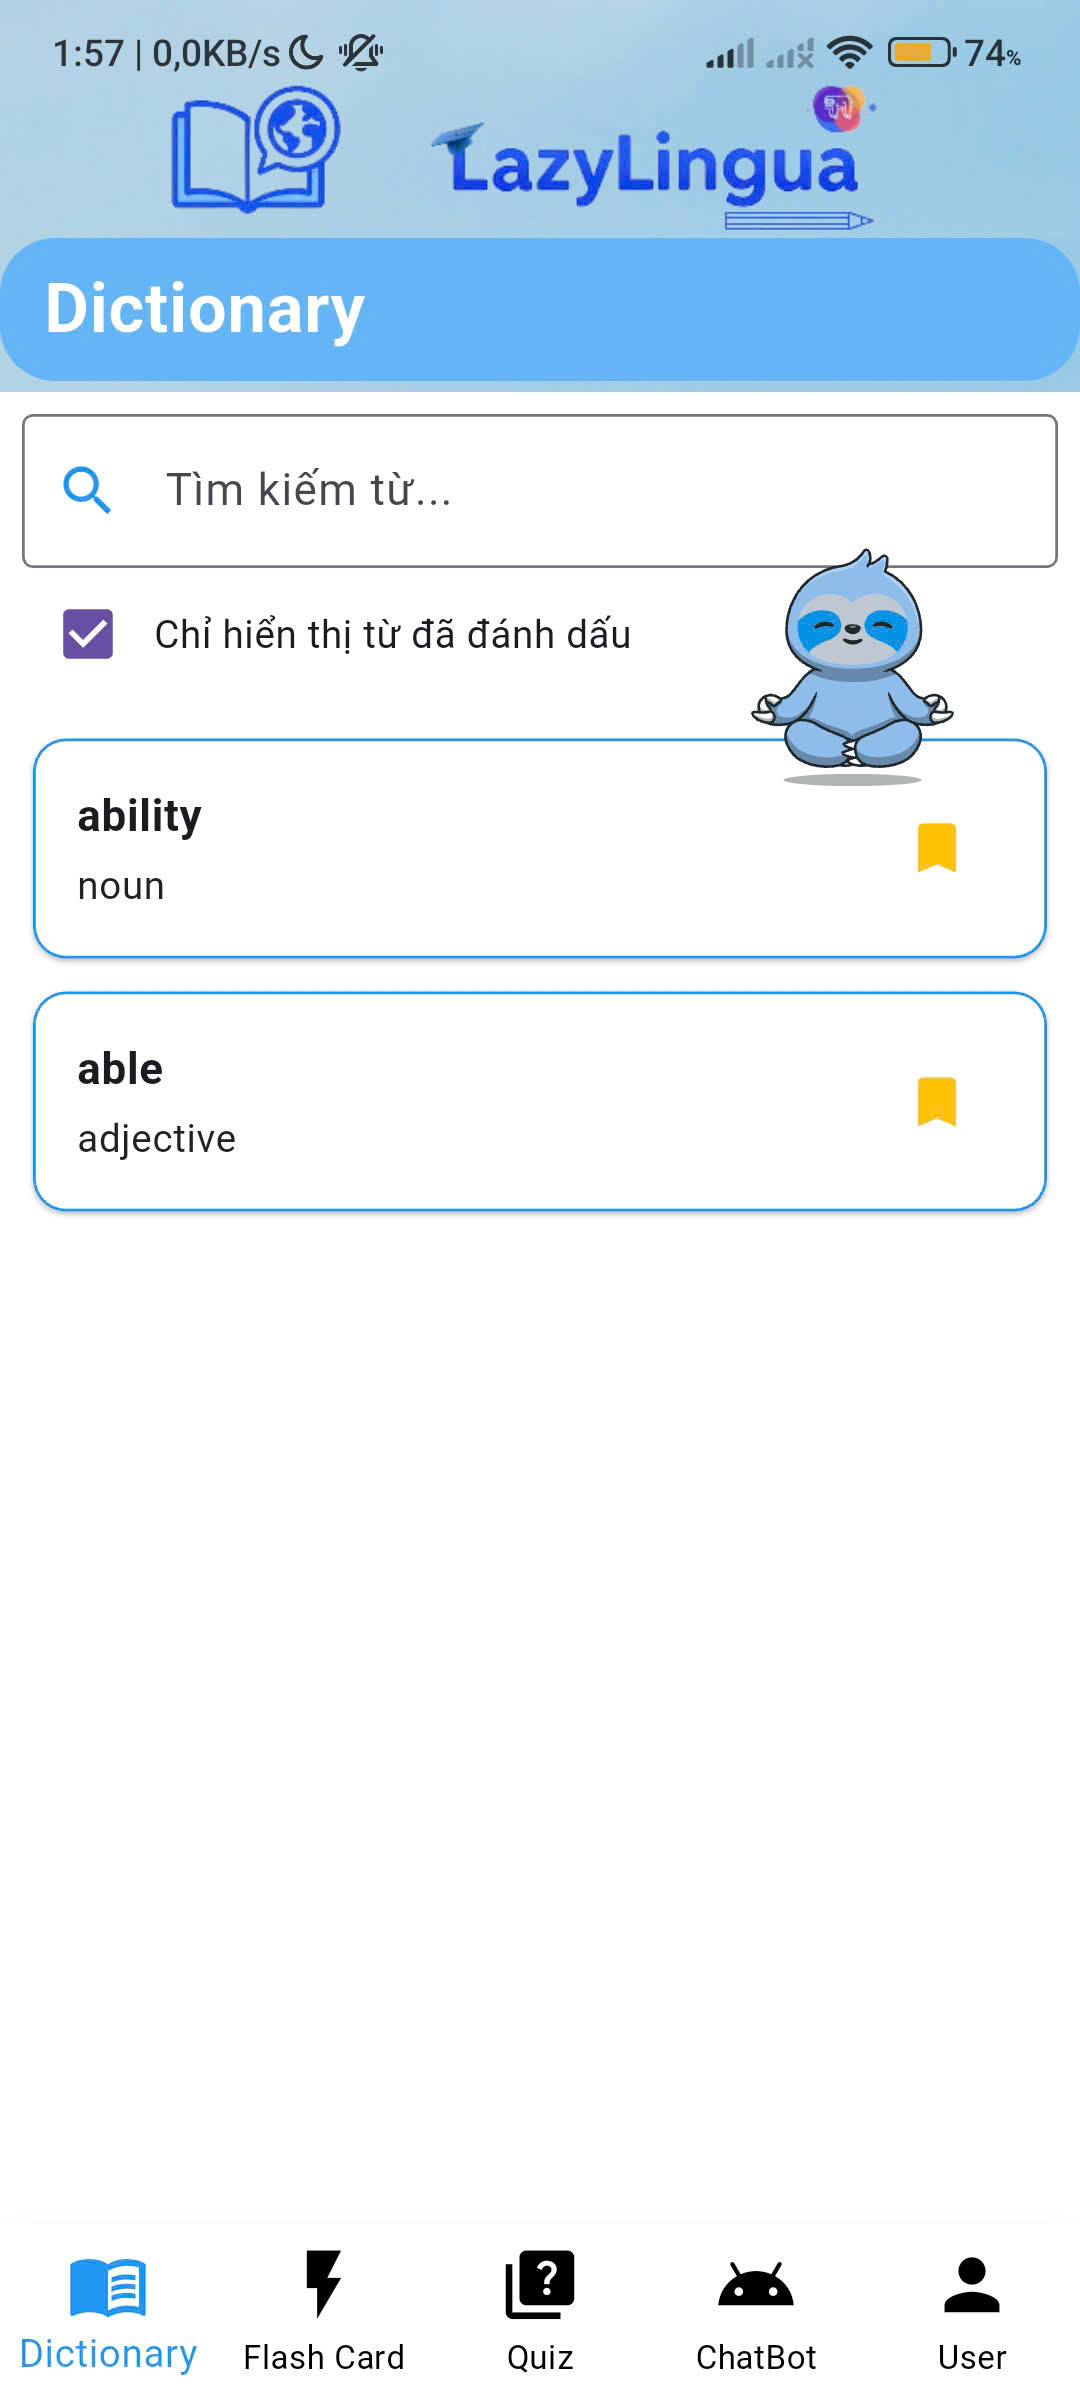
\includegraphics[width=9cm]{ảnh/5.jpg}
\end{center}
\subsection{Màn hình chi tiết từ}
Khi nhấn vào một từ trong danh sách, người dùng được đưa đến màn hình chi tiết. Tại đây sẽ hiển thị định nghĩa đầy đủ, ví dụ sử dụng (nếu có), phiên âm, và nút mở modal dịch. Giao diện thân thiện, dễ đọc, hỗ trợ kéo xuống để tra nghĩa khác.
\begin{center}
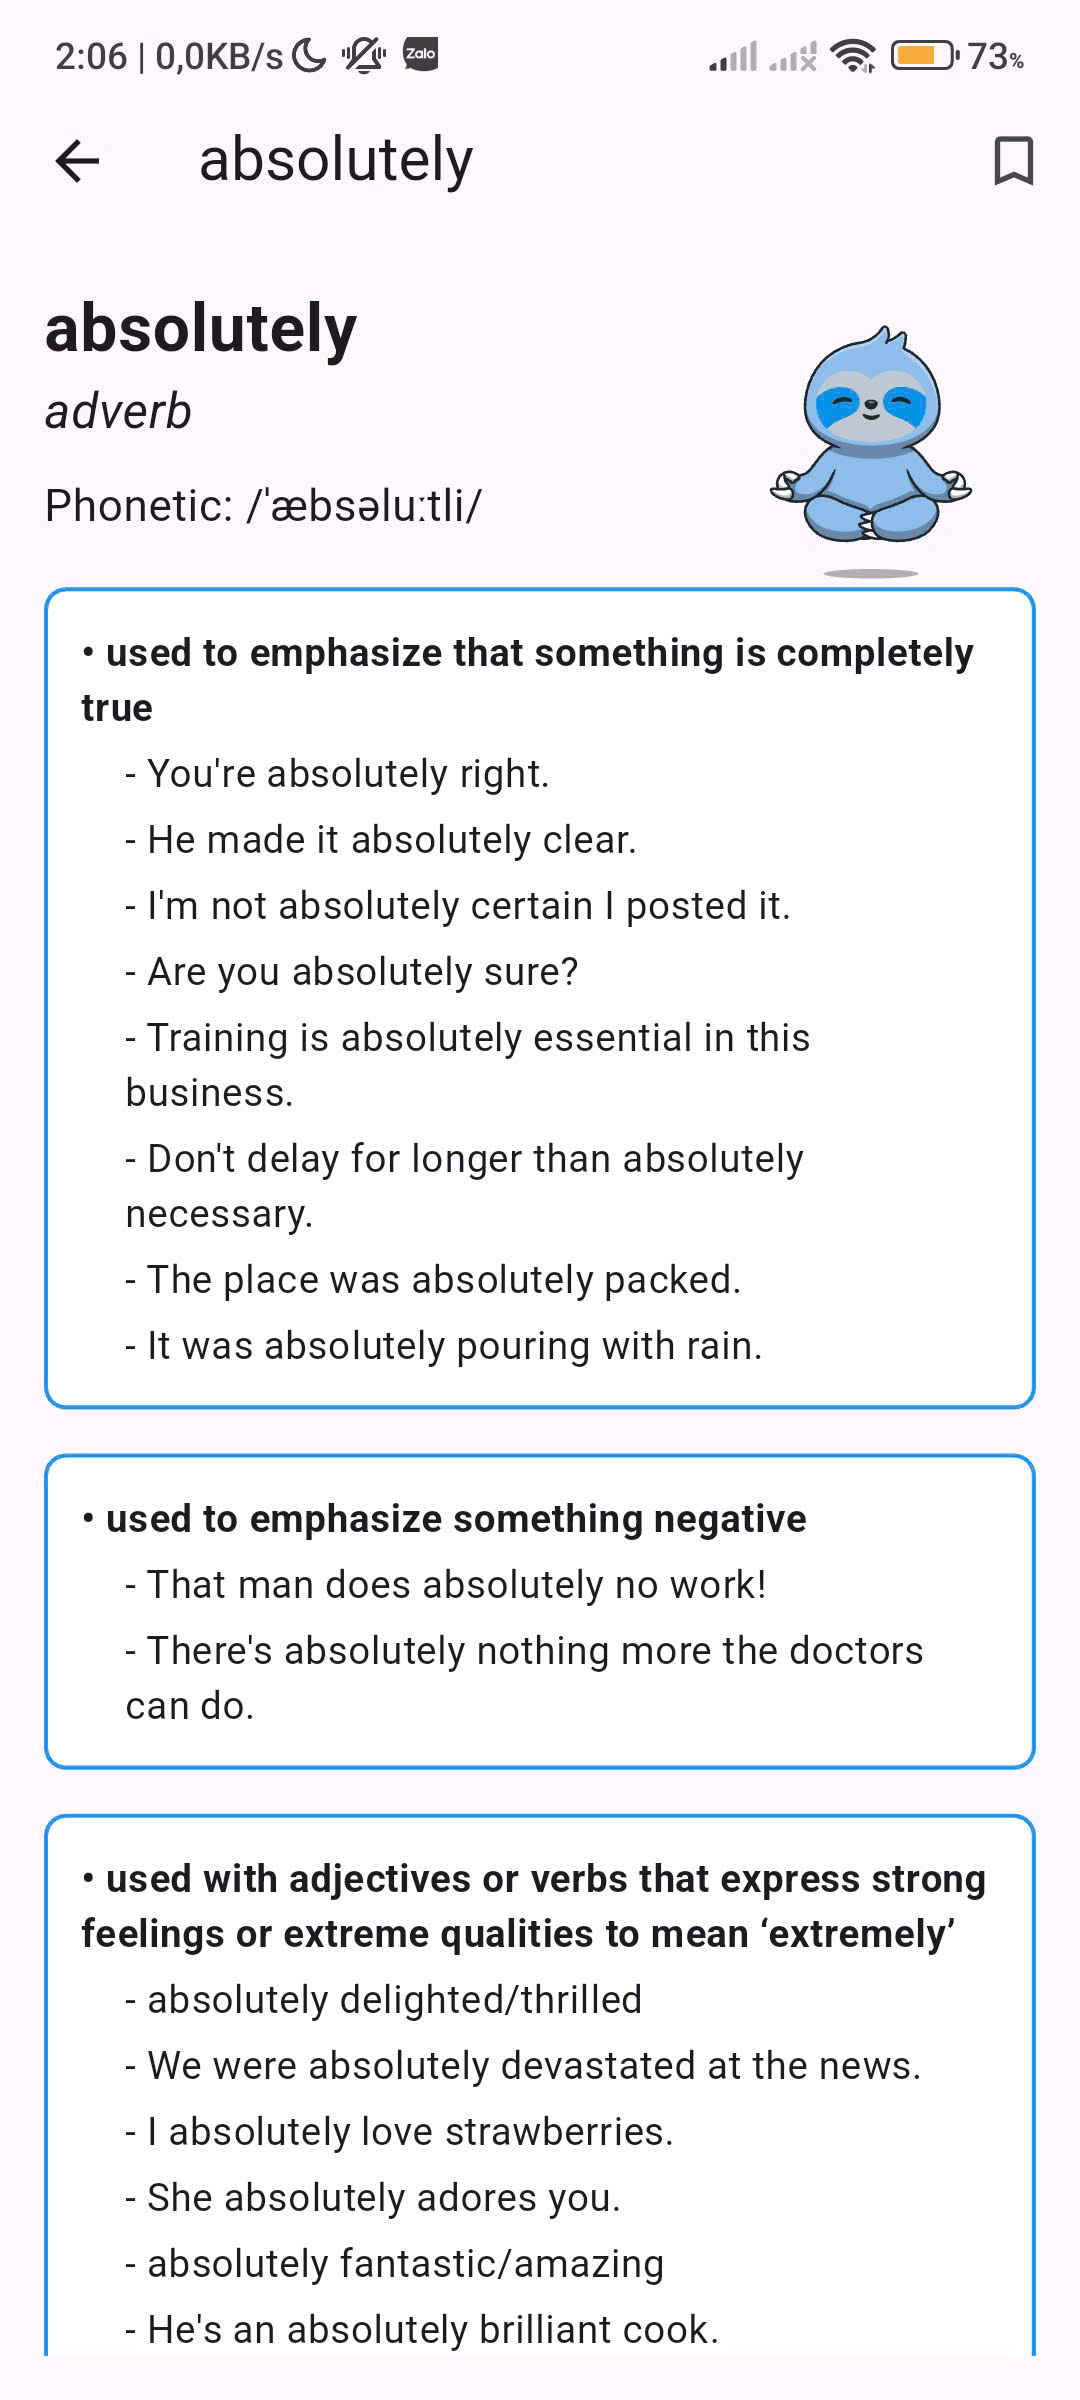
\includegraphics[width=9cm]{ảnh/7.jpg}
\end{center}

\section{Chức năng Flash cards}
\subsection{Màn hình Flash cards}
Flash cards giúp người dùng học từ vựng bằng hình thức lật thẻ. Người dùng có thể nhấn "Next word" để chuyển từ, hoặc nhấn vào biểu tượng bookmark để lưu lại.
\begin{center}
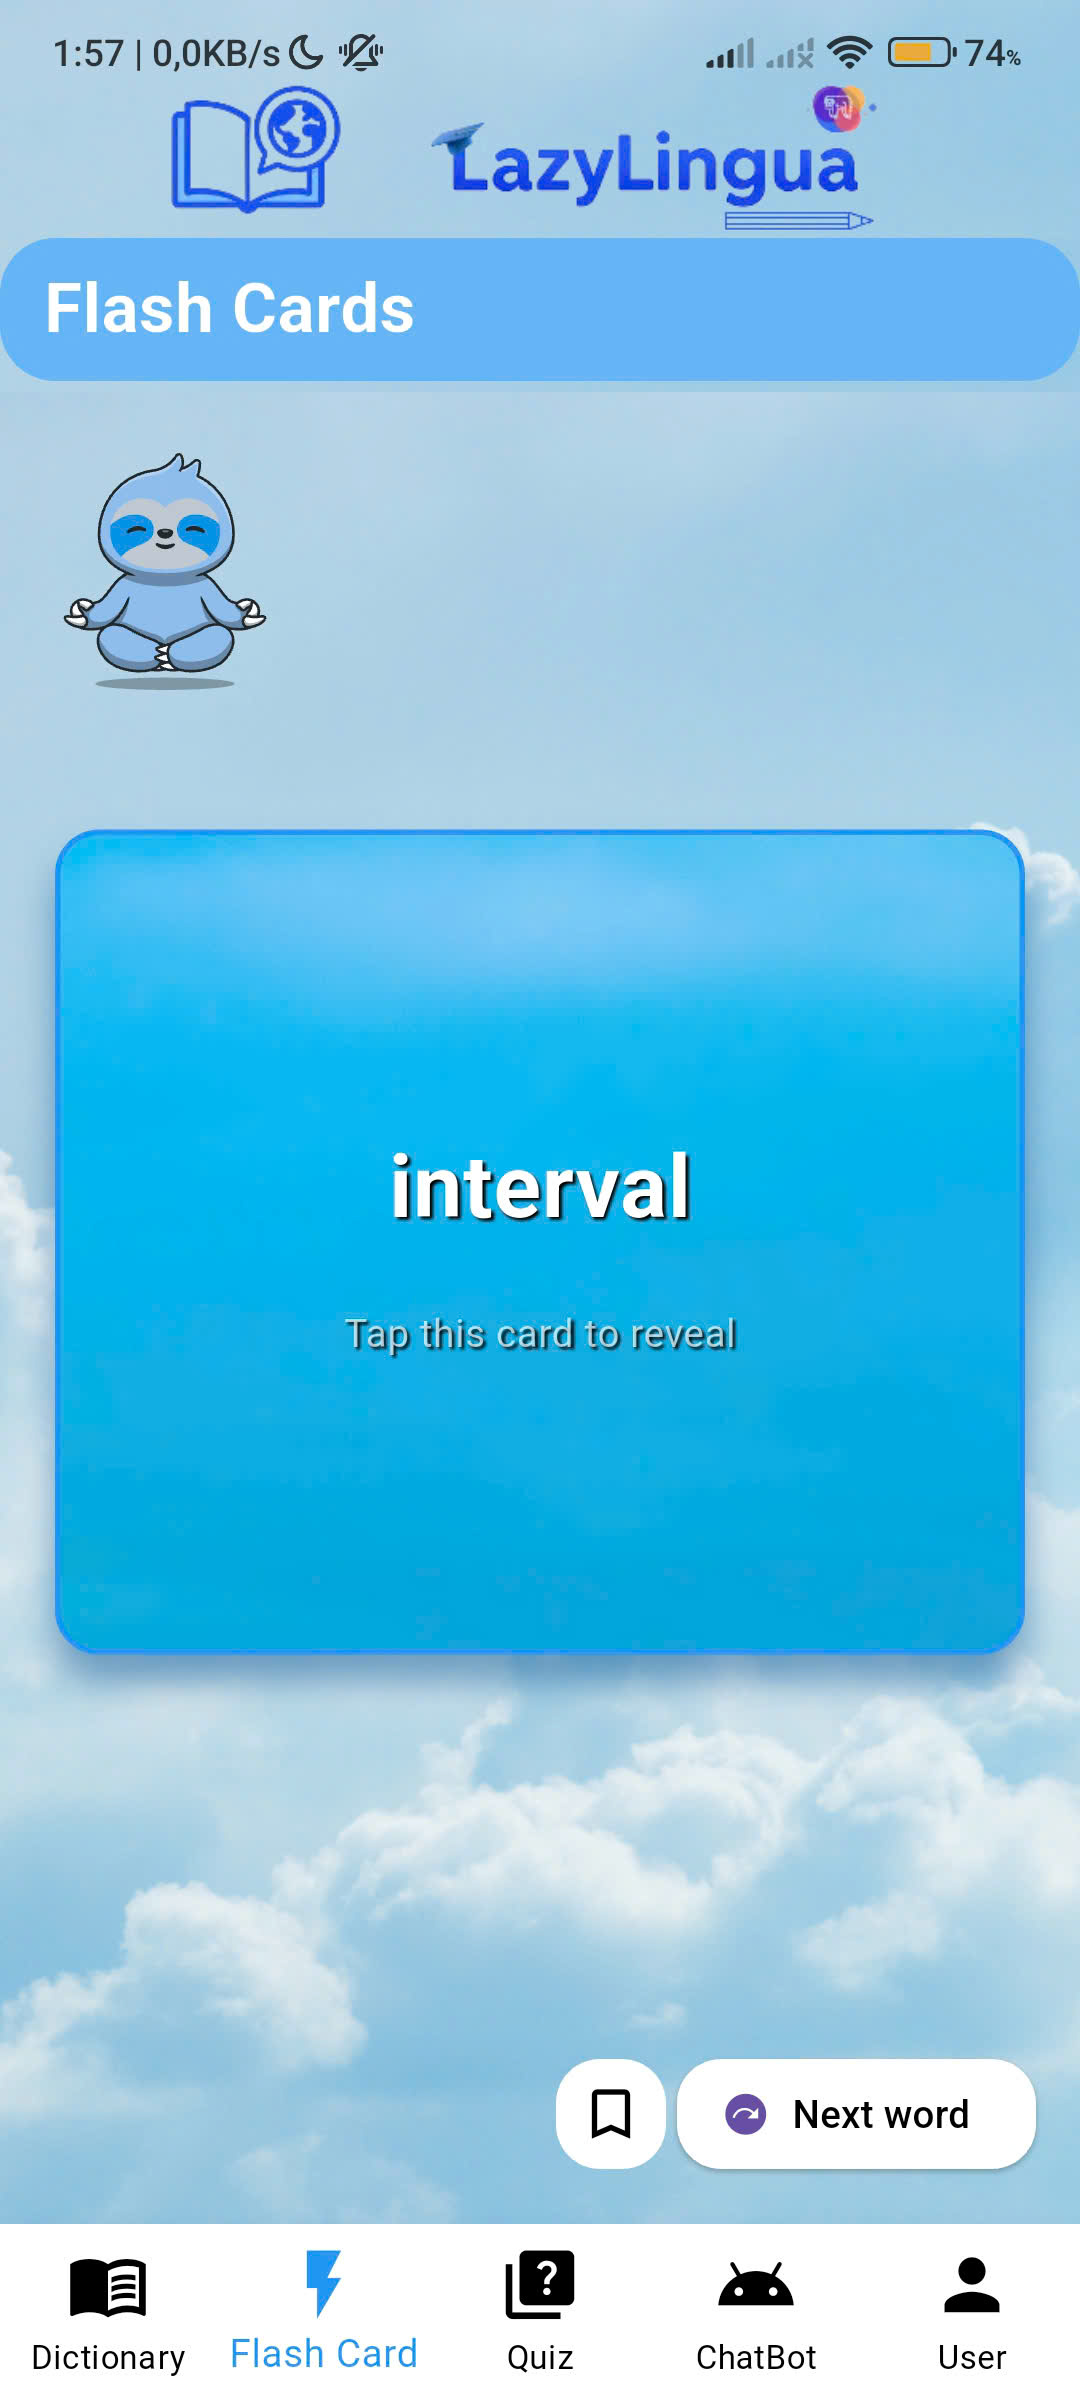
\includegraphics[width=9cm]{ảnh/8.jpg}
\end{center}
\subsection{Màn hình mặt sau Flash cards }
 Khi nhấn vào thẻ, mặt sau sẽ lật lại mỗi thẻ sẽ hiển thị một từ vựng, phiên âm và nghĩa của từ.
\begin{center}
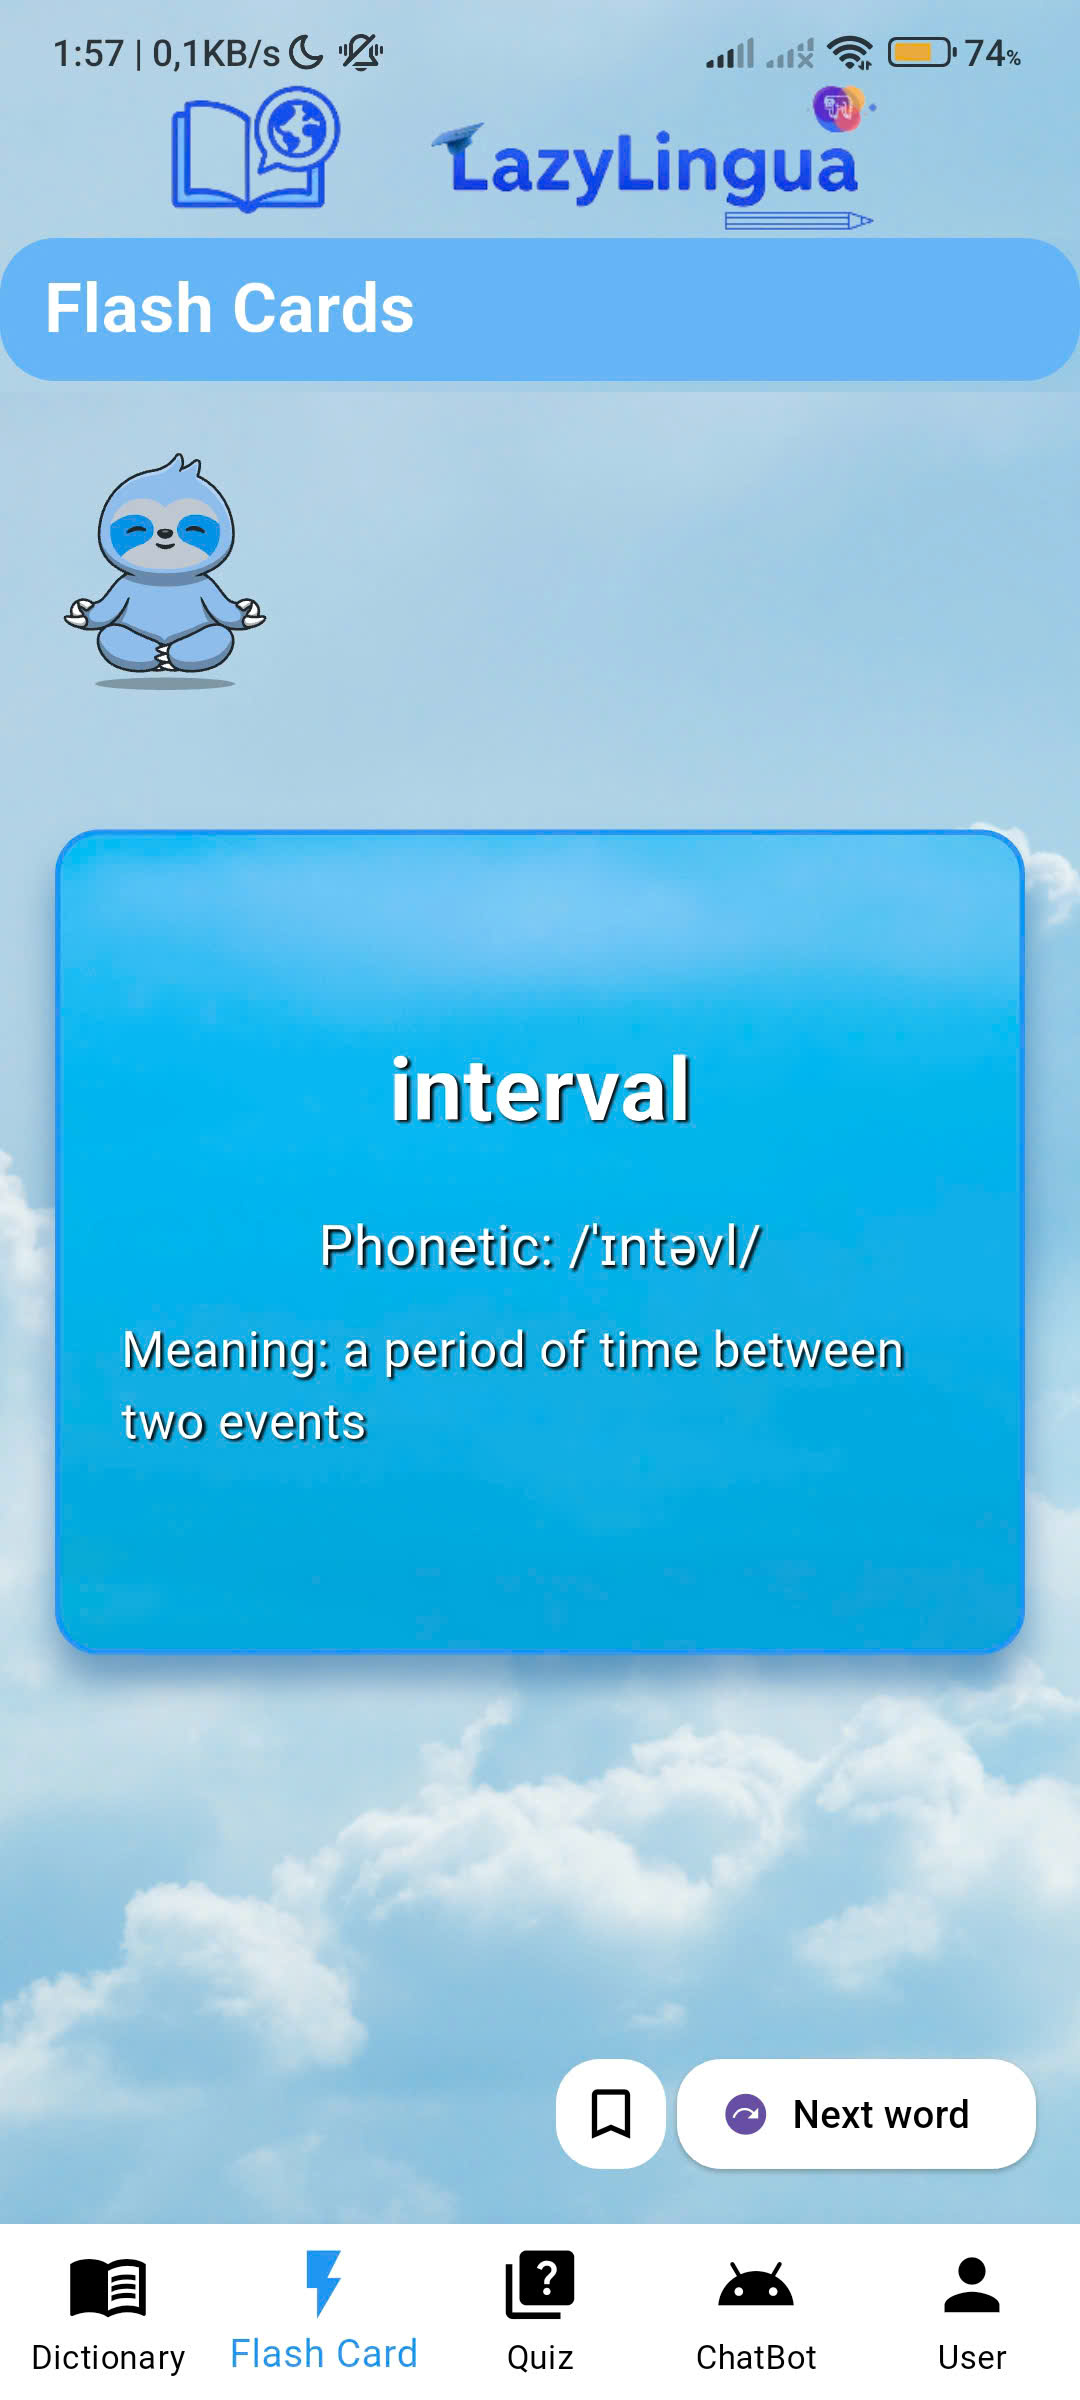
\includegraphics[width=9cm]{ảnh/9.jpg}
\end{center}

\section{Chức năng Mini Quiz}
\subsection{Màn hình câu hỏi}
Mini Quiz là trò chơi trắc nghiệm giúp người dùng ôn lại từ vựng đã học. Mỗi câu hỏi sẽ hiển thị định nghĩa và yêu cầu người dùng chọn đúng từ. Giao diện hấp dẫn với nền ảnh, hệ thống tính điểm và quản lý streak.
\begin{center}
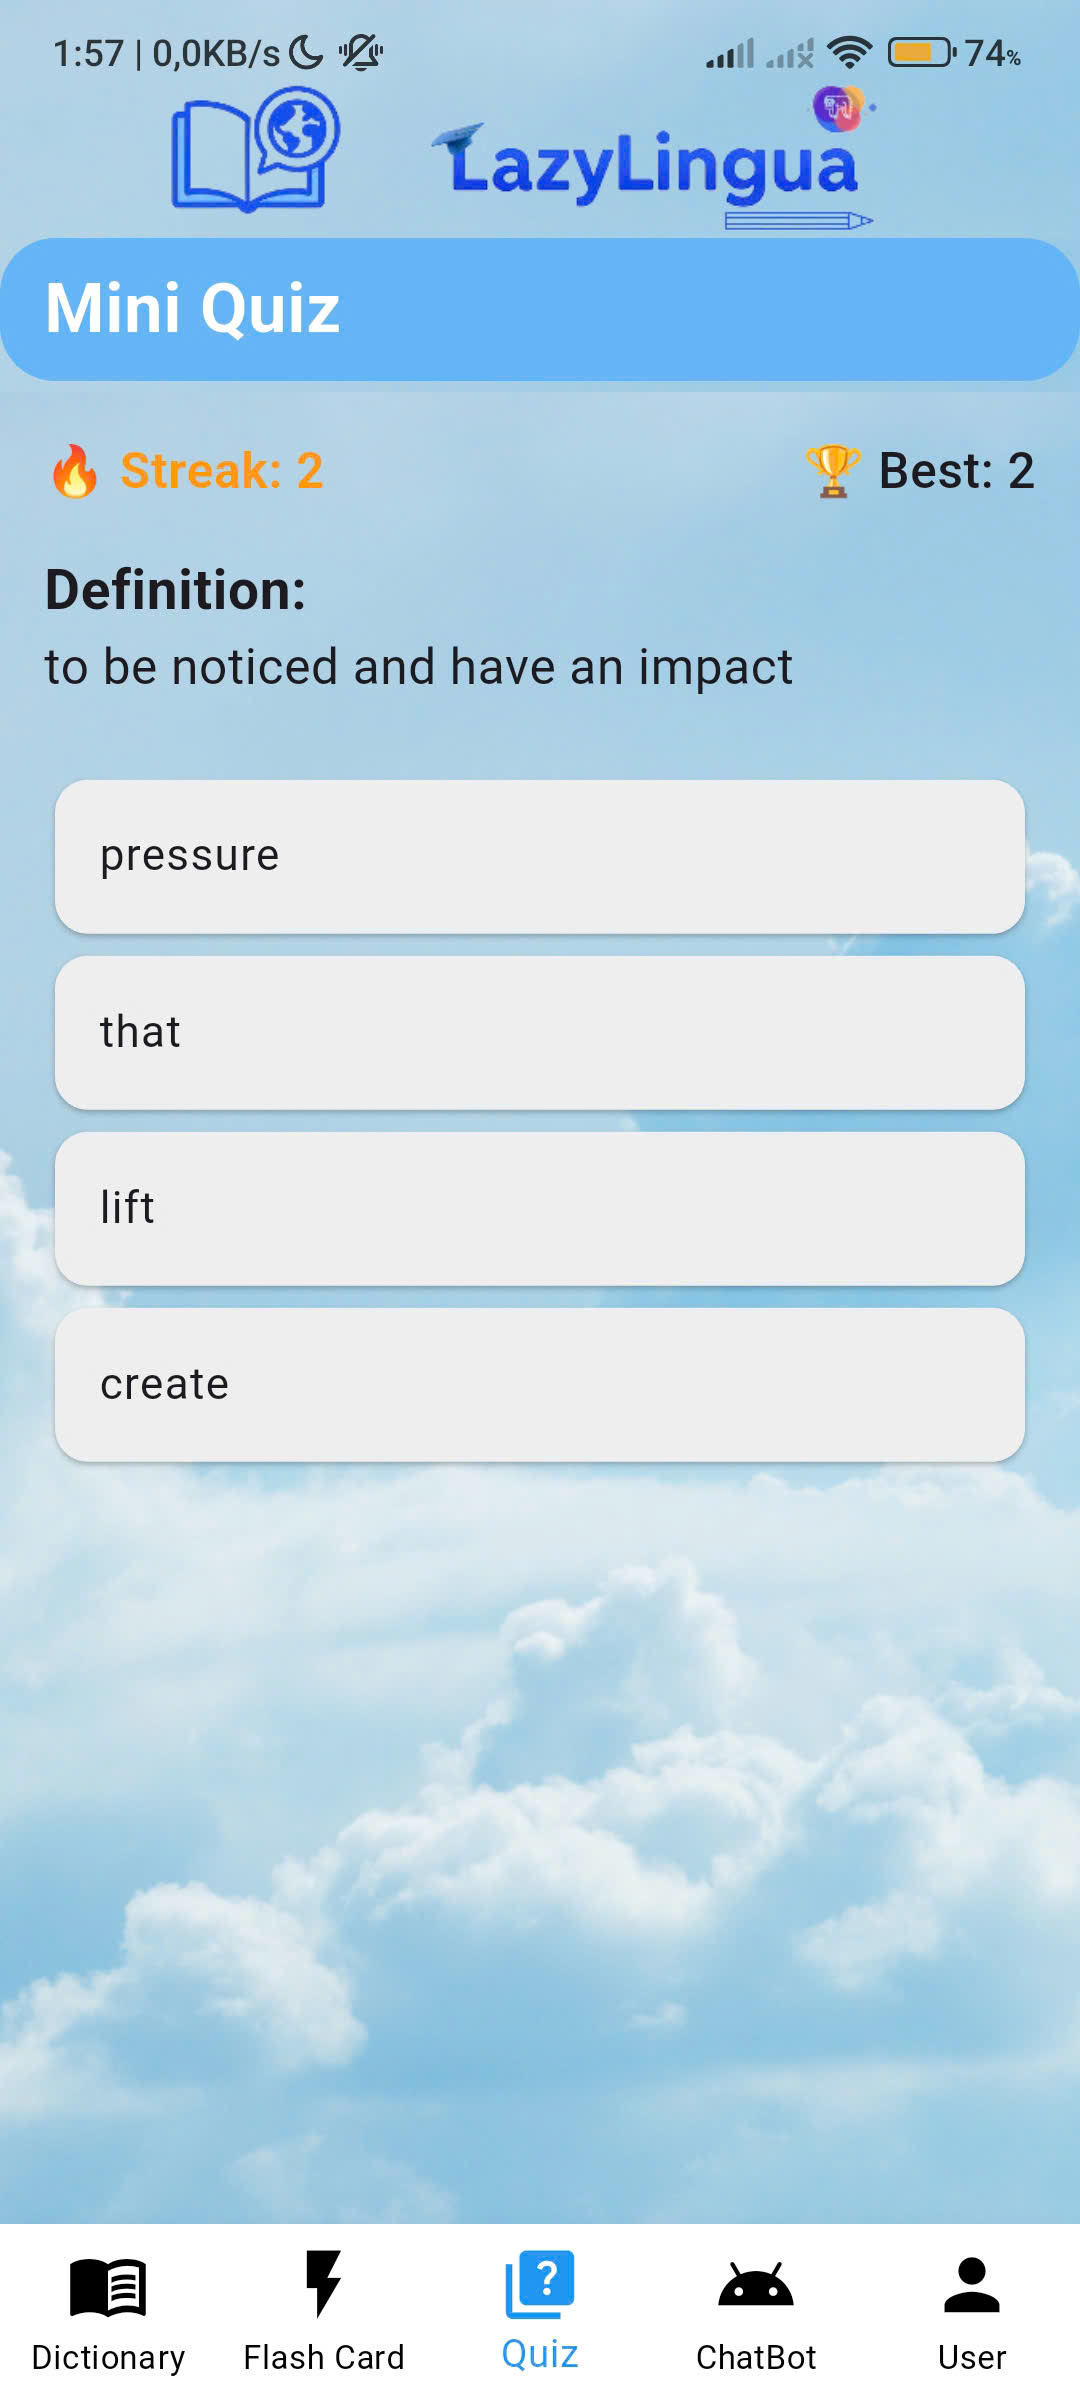
\includegraphics[width=9cm]{ảnh/10.jpg}
\end{center}
\subsection{Màn hình trả lời đúng}
Khi người dùng chọn đúng từ, hệ thống hiển thị màu xanh lá cây kèm hiệu ứng. Streak hiện tại được tăng lên và ghi nhận. Nếu vượt qua streak cao nhất trước đó, hệ thống sẽ lưu lại mốc mới sẽ lưu lại vào local và khi thoát ứng dụng hoặc đăng xuất sẽ lưu vào firestore.
\begin{center}
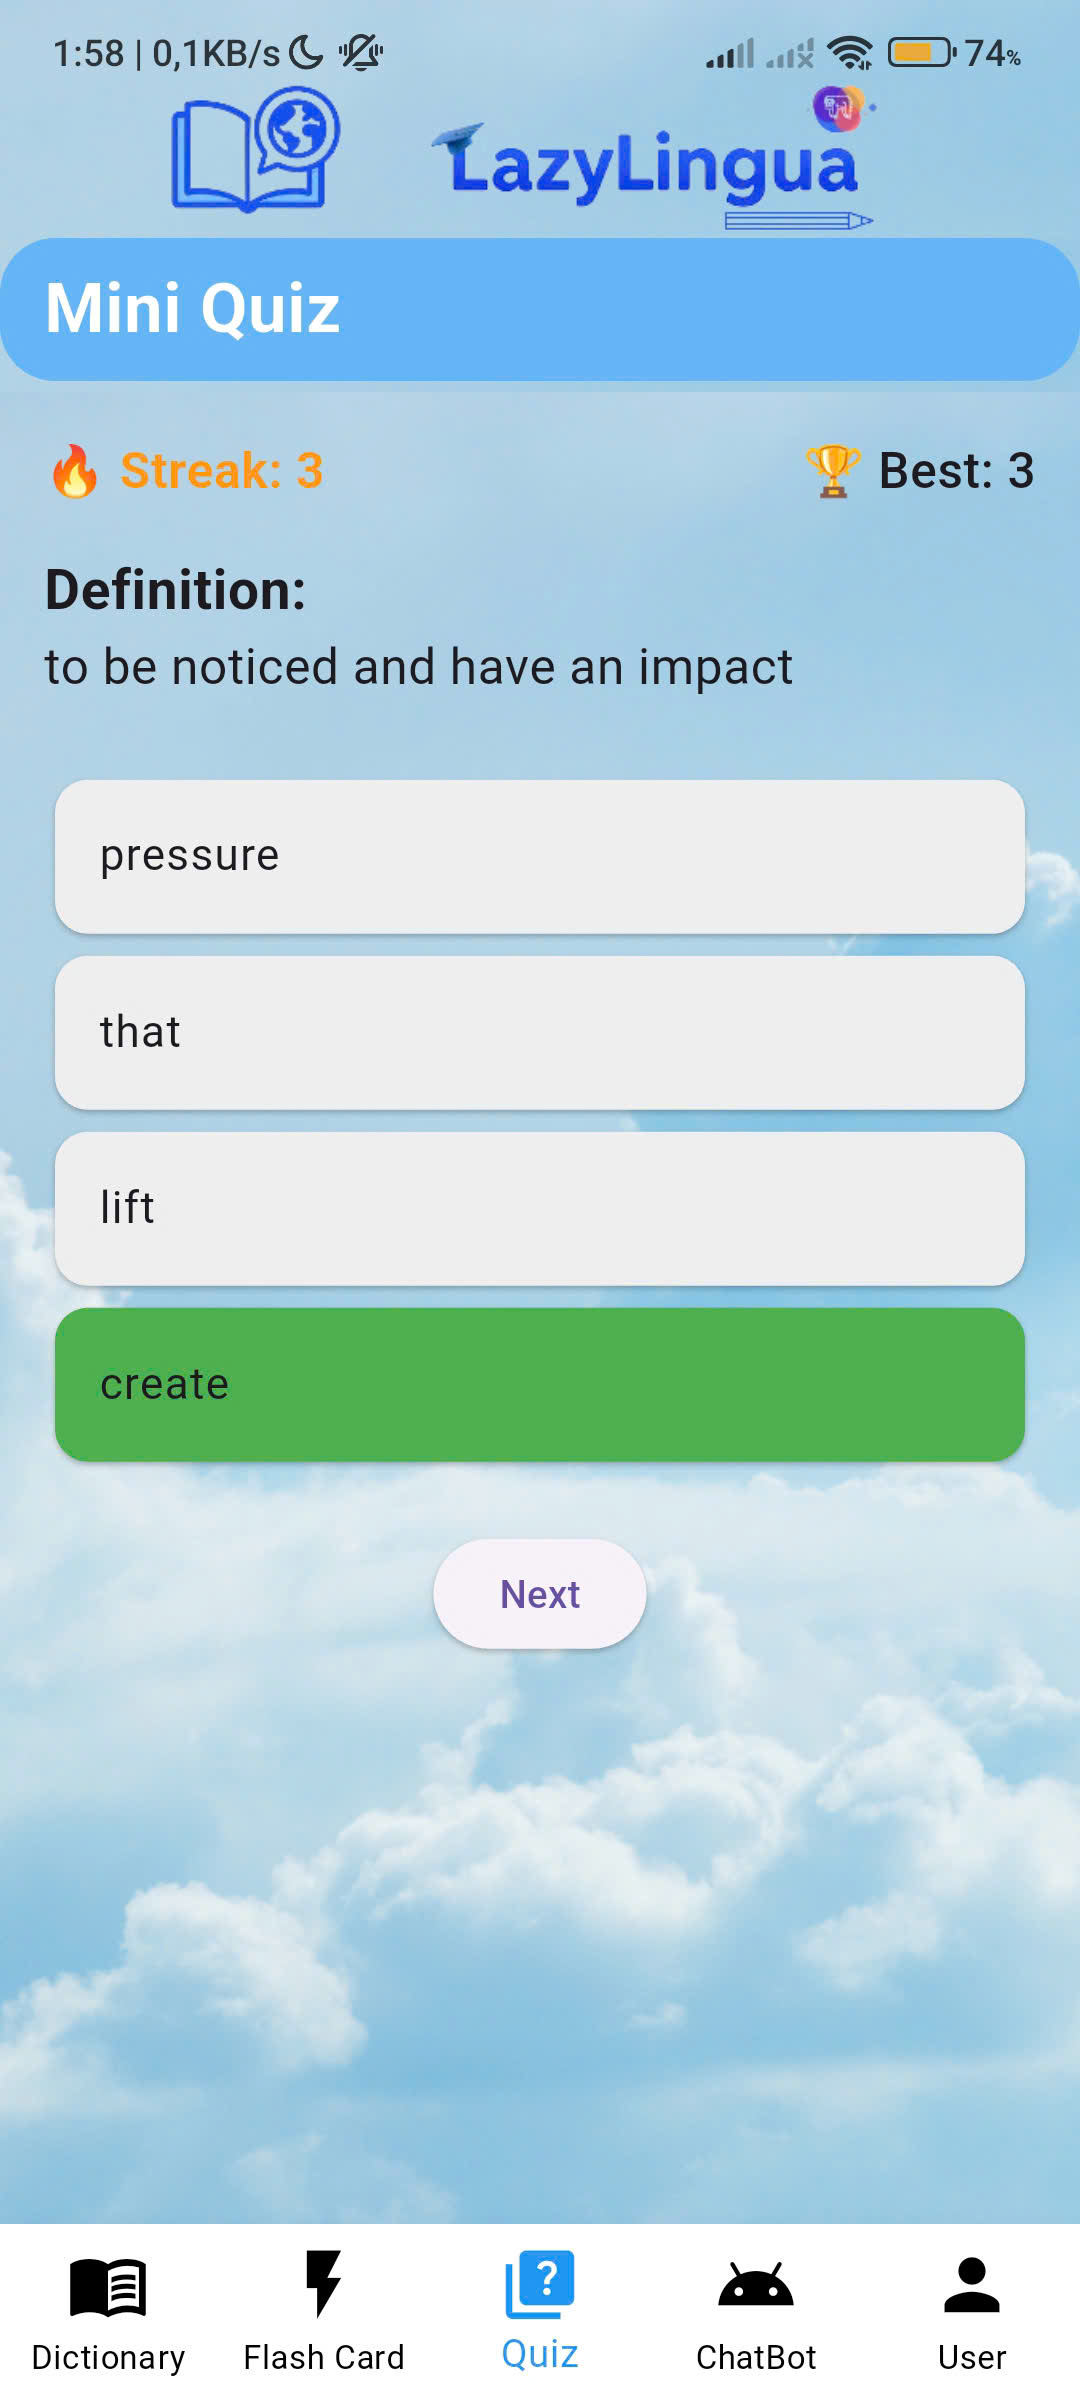
\includegraphics[width=9cm]{ảnh/11.jpg}
\end{center}
\subsection{Màn hình trả lời sai}
Khi chọn sai, ứng dụng hiển thị màu đỏ và cho biết từ đúng. Đồng thời, streak hiện tại bị reset về 0. Tính năng này giúp người học có động lực ôn tập đều đặn để giữ chuỗi streak.
\begin{center}
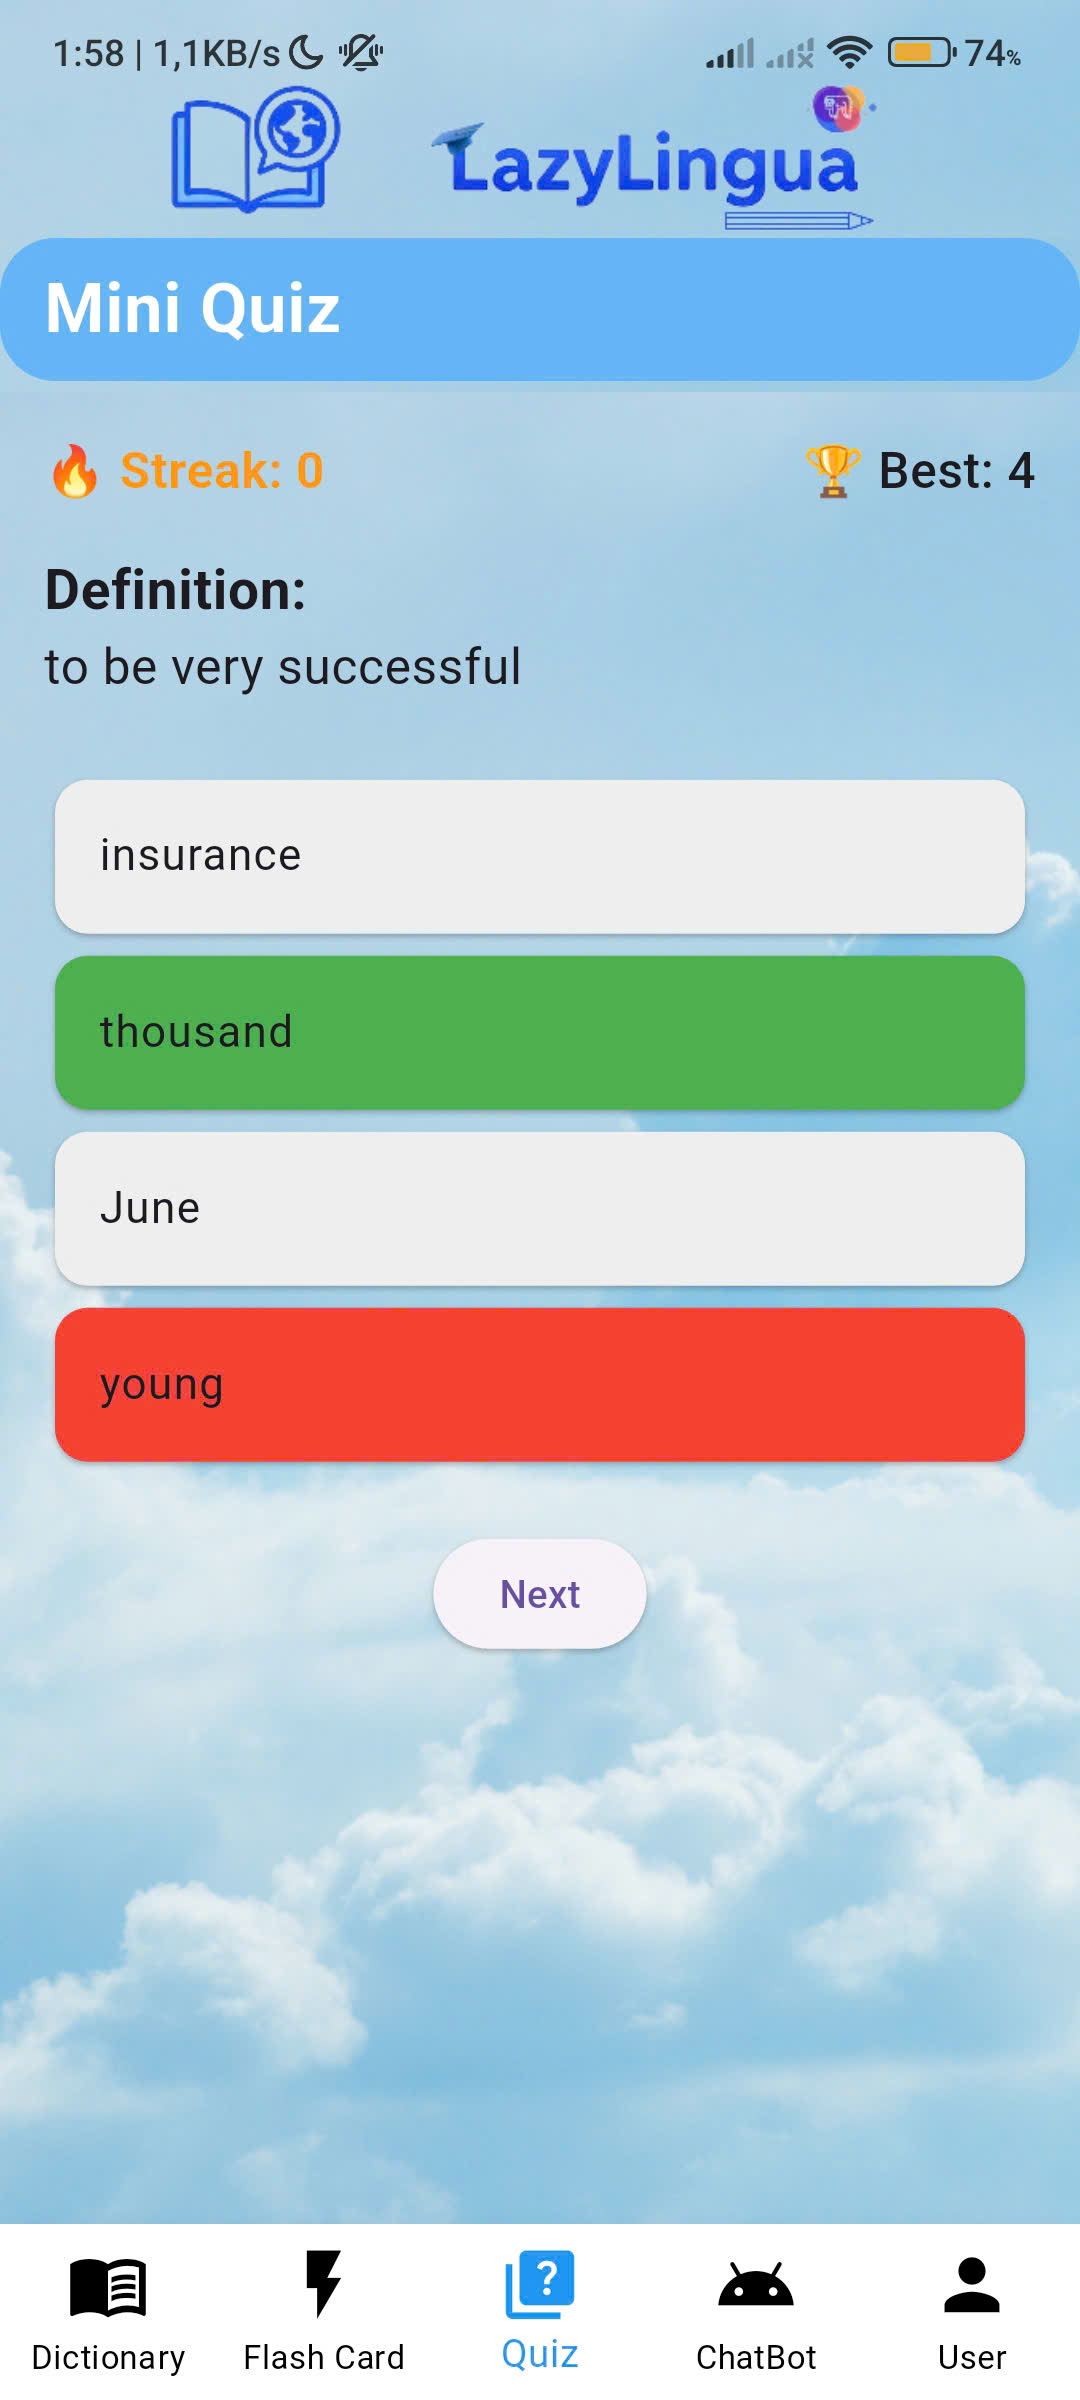
\includegraphics[width=9cm]{ảnh/12.jpg}
\end{center}

\section{Chức năng ChatBot AI}
\subsection{Màn hình ChatBot AI}
Người dùng có thể tương tác với AI chatbot tích hợp GPT để luyện nói hoặc đặt câu hỏi về từ vựng, ngữ pháp. Lịch sử chat được lưu bằng SharedPreferences và giữ trạng thái giữa các lần sử dụng. Giao diện bắt mắt với ảnh nền và khung chat giống ứng dụng nhắn tin thực tế.
\begin{center}
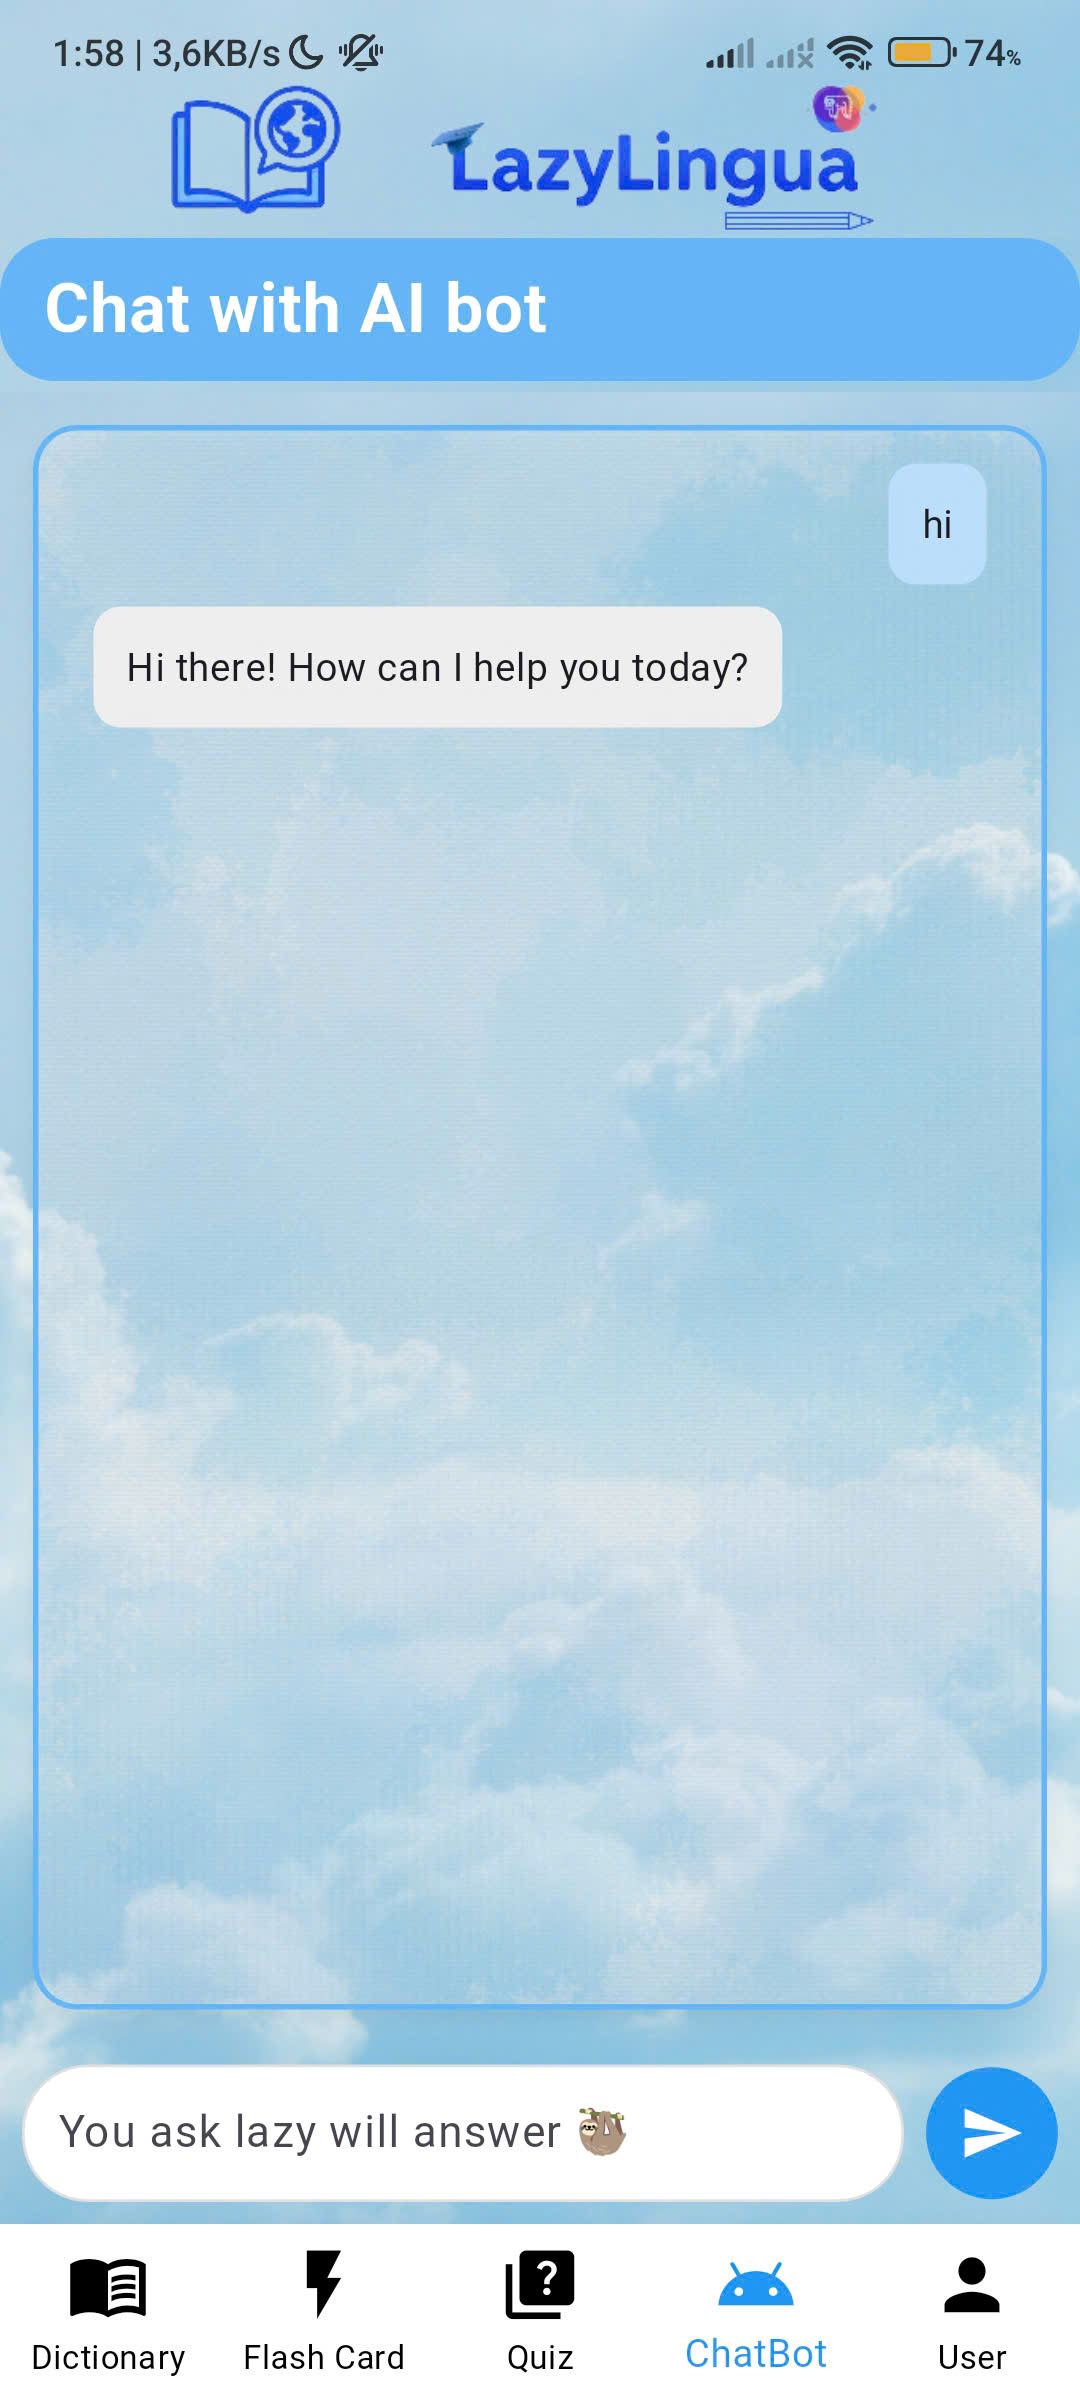
\includegraphics[width=9cm]{ảnh/13.jpg}
\end{center}

\section{Chức năng dịch ngôn ngữ}
\subsection{Màn hình "Lười" Phiên Dịch}
Chức năng này cho phép người dùng nhập đoạn văn bản tiếng Anh, sau đó sử dụng Google Translator để dịch sang tiếng Việt. Modal dịch có hiệu ứng mờ nền, giao diện đơn giản với ô nhập, nút "Dịch", và vùng hiển thị kết quả. Modal có thể mở từ bất kỳ màn hình nào nhờ nút Lottie hình robot “lười”.
\begin{center}
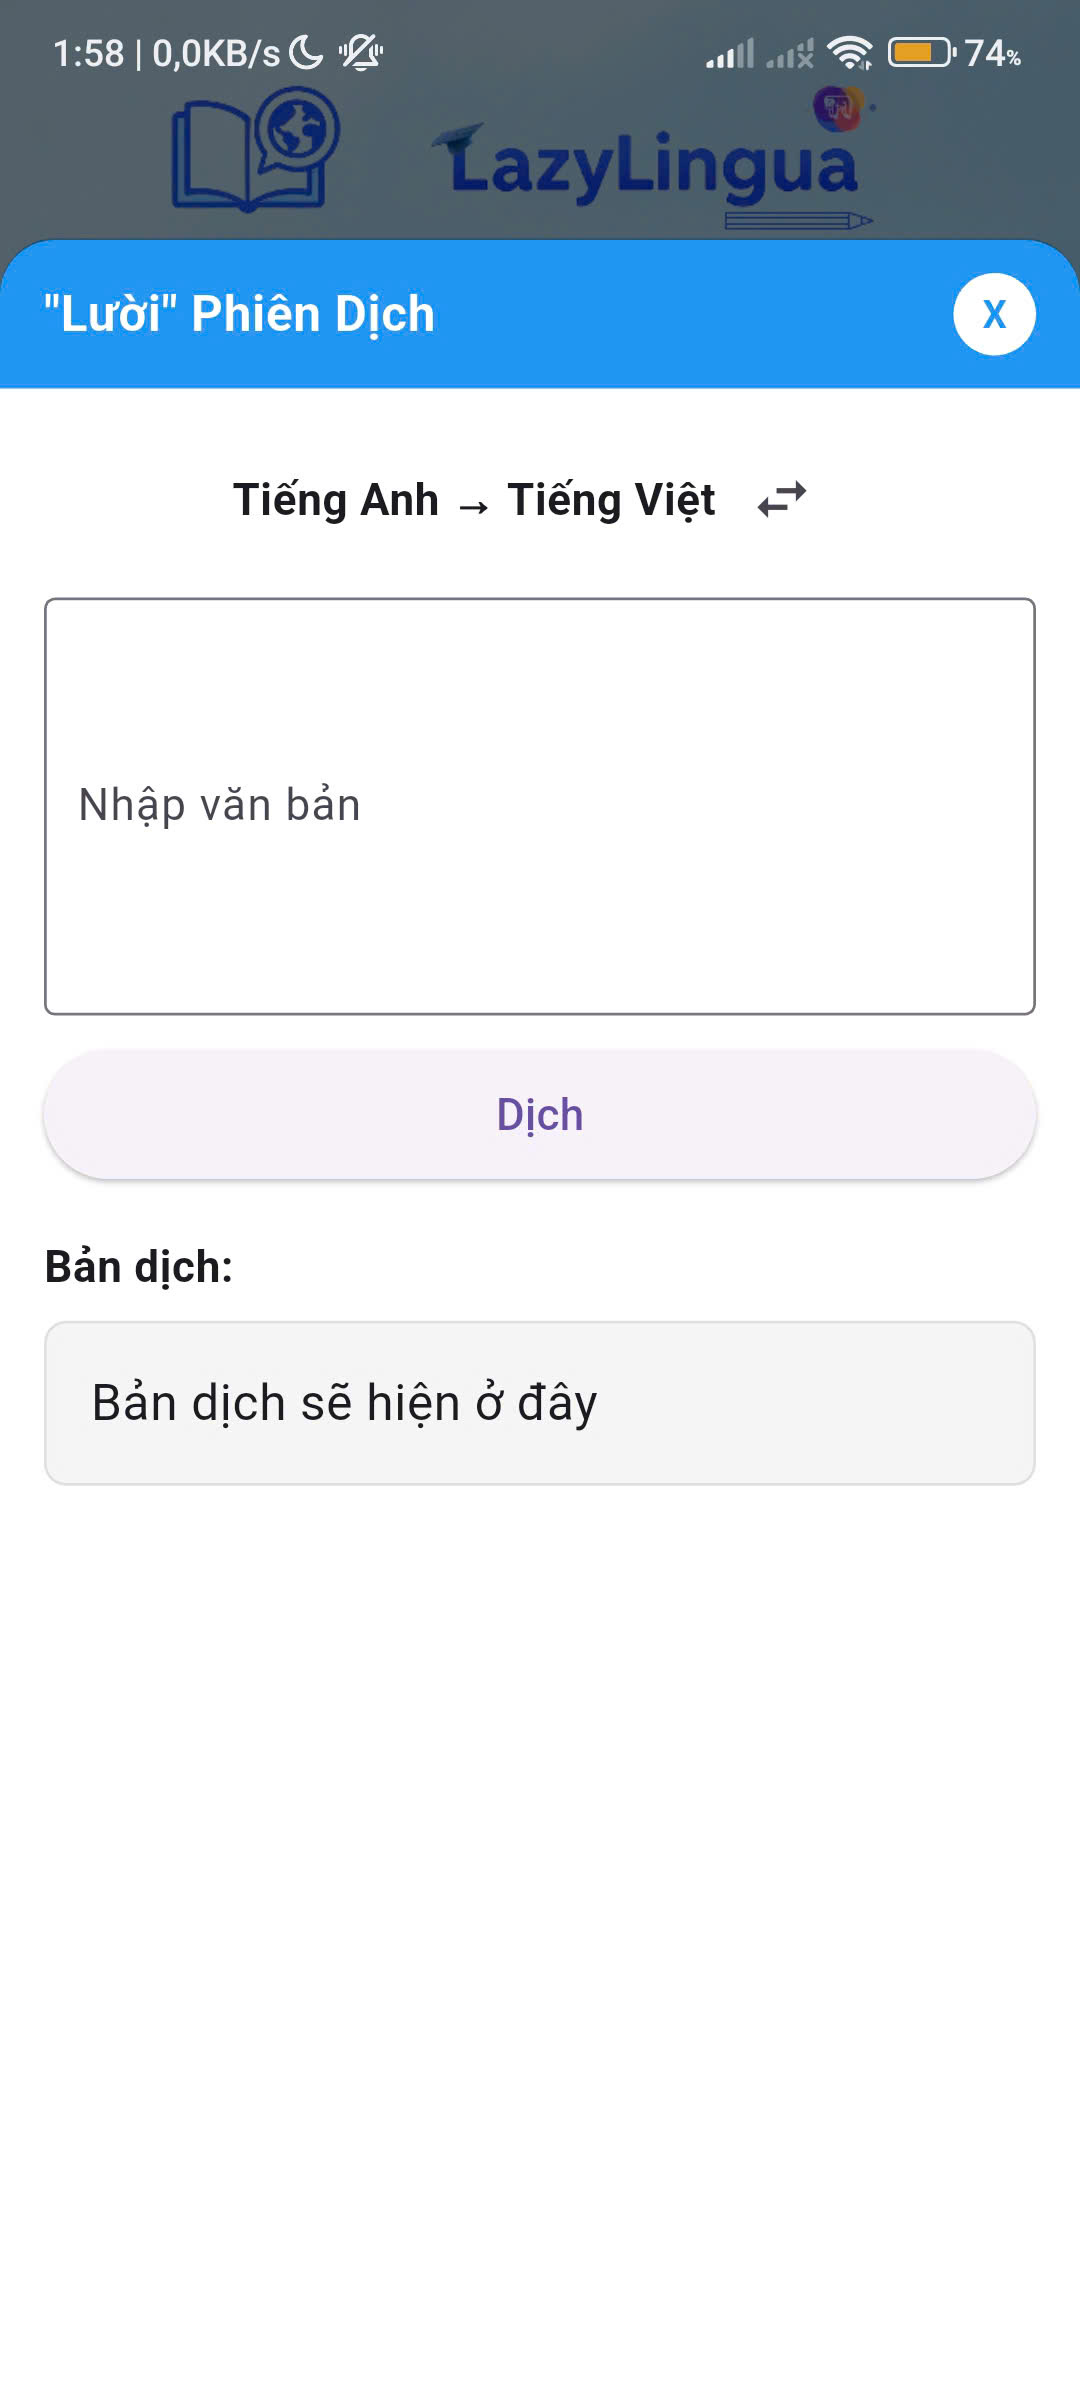
\includegraphics[width=9cm]{ảnh/14.jpg}\\
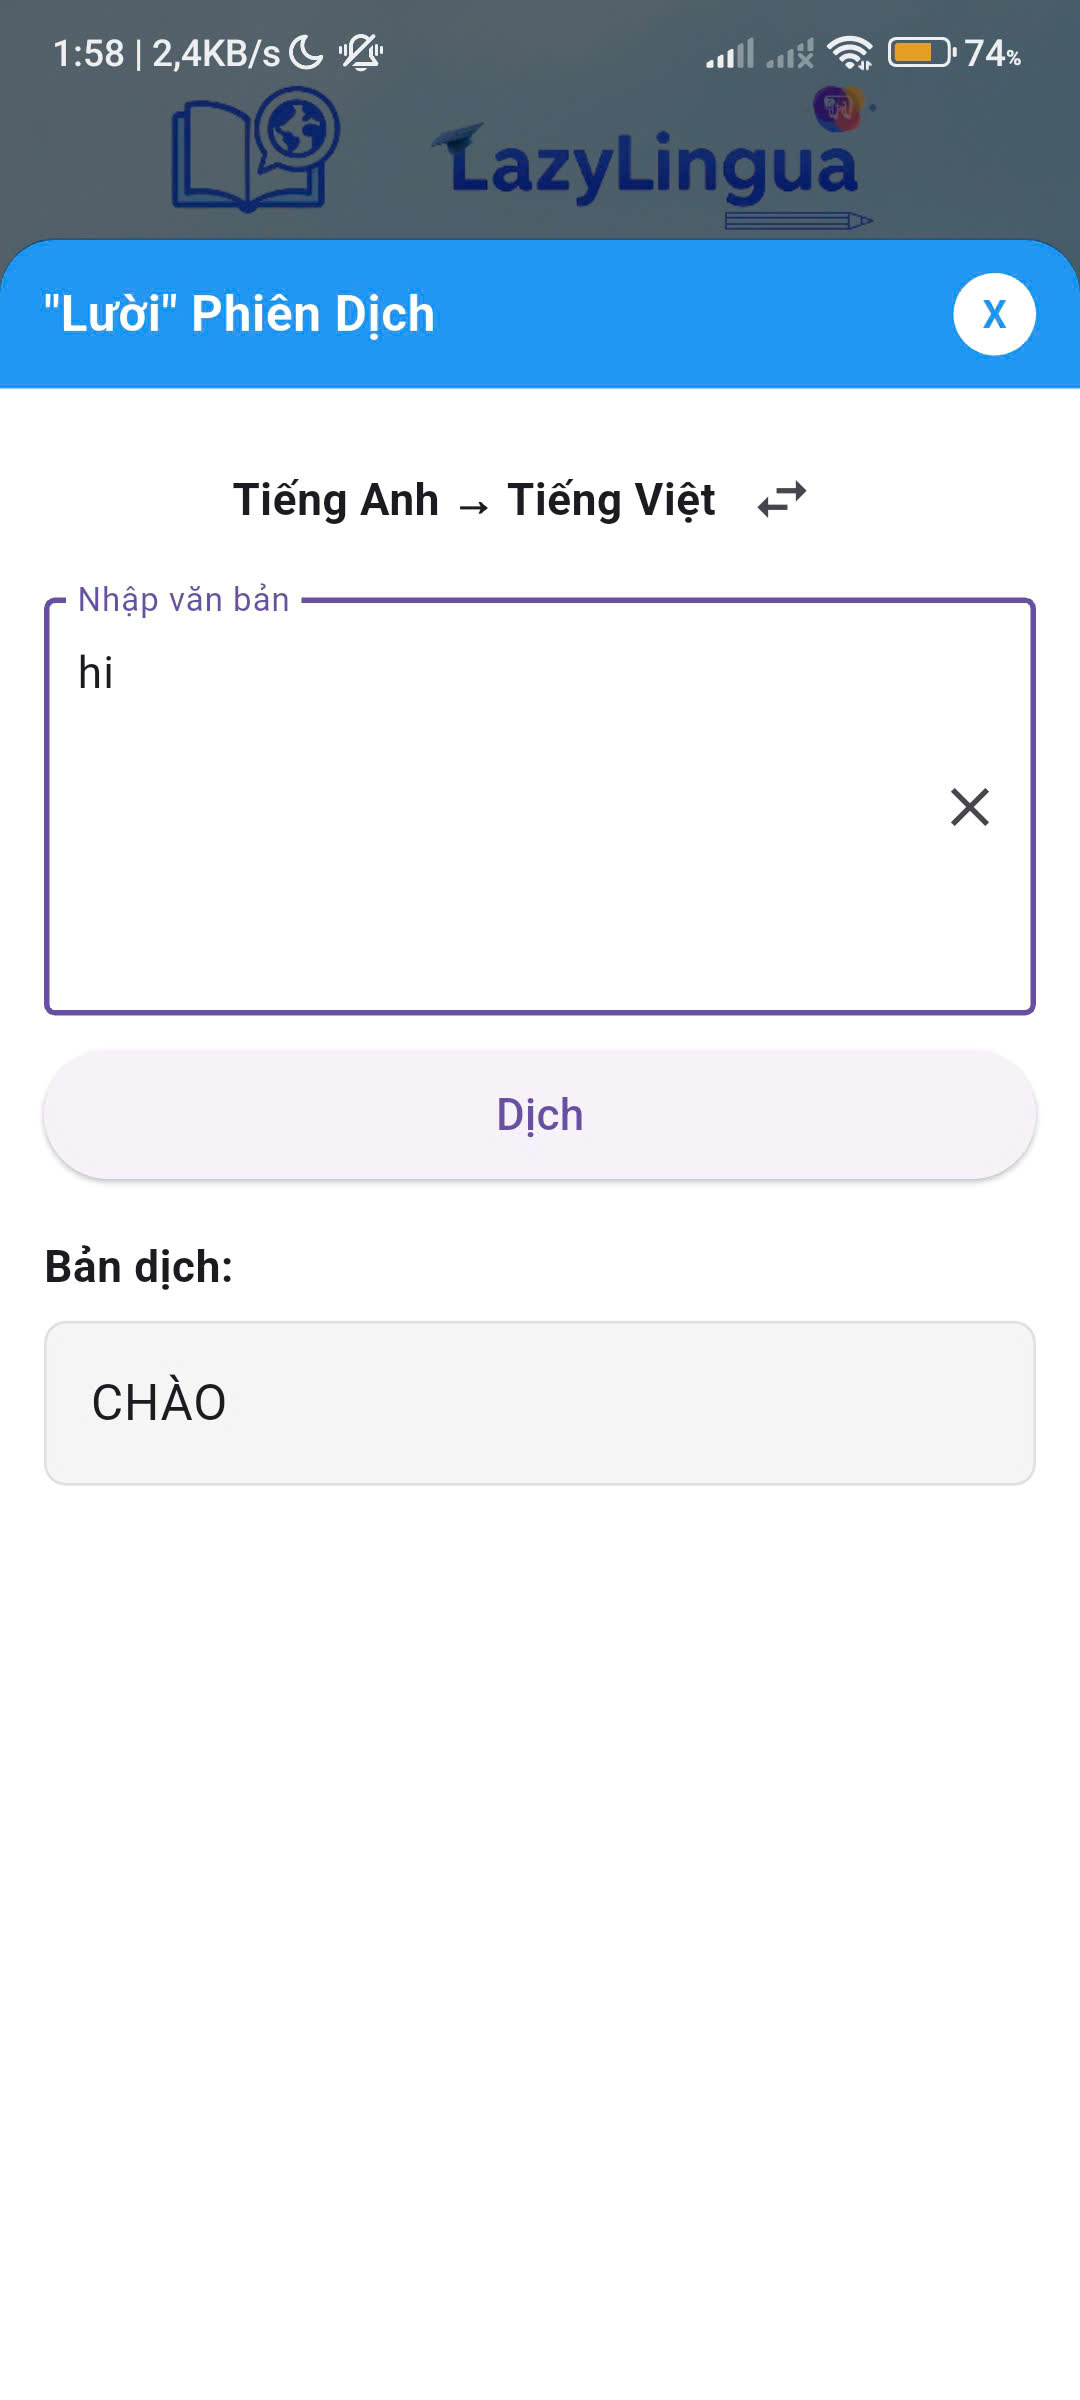
\includegraphics[width=9cm]{ảnh/15.jpg}
\end{center}

\end{document}

